
\chapter{Color Space Methods}

\section{Implementing the Color Space}\label{sec:ImplementingTheColorSpaceApp}

Here, we will outline the practical implementation of the color space algorithm on the mobile device.

The first and most pressing consideration is limited processing power; while our mathematical approach to the algorithm design is significantly faster and more efficient than the more typical color space algorithms --- as will be discussed in the following chapter --- minimizing the number of clock cycles spent on continuous processes is necessary in order to ensure efficient operation. In the case of redistribution, the integer matrix transform is performed first, which puts the pixel values in the quantized working type $qRsRange$ described in Chapter 2, then pixel classification is performed before any of the chromatic information is redistributed as illustrated in Figure \ref{fig:PartitioningRegions}.

The pixel classification is performed before the redistribution because it excludes processing pixels which are of no interest based on both chromatic channels, whereas for redistribution one channel may clearly lie outside of the discard region $\lambda$ while the other could be kept or redistributed. With the pixel classifier, if one channel lies outside the discard region, the other is also of no interest since the pixel value is outside of the partitioning region, thereby avoiding unnecessary processing time spent on redistribution. The classification is straightforward within the limits on the channel values, so it isn't sophisticated like an elliptical partitioning or a probabilistic Gaussian-based thresholding; it is simply a quick way of excluding the majority of the pixel values which aren't of interest.

Once the pixels have been classified, the redistribution is performed --- which requires further processing --- or we assign a pixel value from a small set of possibilities and skip onto the next pixel value. The redistribution function is applied to the working type $tRange$, while the comparison and classification is done in $qRsRange$. This is because the information in $tRange$ is compressed to avoid wasting space, and as a consequence of this it does not occupy the full data type. $qRsRange$, on the other hand, being the natural range multiplied by the quantization matrix qR, does occupy the full data type. Since the operation is simply a comparison between numbers, it is of no advantage to compress the information so tightly. Additionally, since $qRsRange$ is a signed range, one could look at the bit indicating the sign and immediately tell whether or not a given value will be discarded. Once scaled to $tRange$, the redistribution function is applied --- which has a source range of $tRange$ and a range $dRange$ of the destination type --- as outlined in Appendix \ref{app:PreservationOfColorInformation} in Chapter 2.

It should be noted that the region between the extended keep region $\omega p$ and the discard region $\lambda$ is not especially large; for even a $5\sigma$ result, it's only tens of values wide. As such, we use a lookup table for the redistribution in our actual implementation, thus further reducing the processing overhead. The C++ implementation has a lookup table threshold set to 64, a quarter of the source data type range. If the redistribution region is larger than that, the error function approximation from Chapter 2 is used. This is mainly for future-proofing the implementation; given the limited size of the region, we fully expect to use a lookup table for all practical cases.

As another future concession, the facility to add pixel-based functions to the color space transform, such as the skin probability function mentioned at the end of the previous chapter, is allowed. The color space transform is a threaded process, so there is no way of knowing that the last pixel value that was processed by any given thread was an adjacent pixel, as the parallelization is handled by OpenCV's universal threading library implementations. Pixel-based functions, however, are per-pixel processes, and they come out as separate resulting channels, so they can be added to the color space transform without causing any conflicts.



\subsection{The White-Out Black-Out Algorithm}\label{sec:WhiteOutBlackOutAlgorithm}
We need to find the point at which a chromatic value begins to suffer from white-out and black-out. This is done by taking the corresponding RGB value for the chromatic point and illuminating and deluminating the point by shifting the channel values by the same amount, noting when each channel value becomes fully saturated or desaturated. This is done in the unit space so the results can be scaled to any working range. The algorithm for finding the theoretical values is given in Algorithm \ref{algo:TheWhiteoutBlackoutAlgorithm} below. 

\begin{algorithm}[H]
 \begin{algorithmic}
  \Require{ $Ca$, $Cb$ The chromatic values}
  \State \phantom{Require}  { $iLCaCb$ the transform to LCaCb from RGB; }
  \State \phantom{Require}  {  $LCaCb$ the transform to RGB from LCaCb}
 \Ensure{  The luminosity at which black out $L_{BO}$  and white out $L_{WO}$ occur.}
 \State \phantom{Ensu} { \begin{tabular}{l}
 $Ca_{min}  \le Ca \le Ca_{max}$   \\ 
 $Cb_{min}  \le Cb \le Cb_{max}$  
 \end{tabular}  \parbox{0.65 \textwidth}{The chromatic range which could be suffering from white-out or black-out}}
 
   \State  $pnt^{RGB} \gets iLCaCb(0.5, Ca,Cb)$ \Comment{Put the point in RGB space }
   \State  $O \gets Order(pnt^{RGB}, \#1> \#2)$ \Comment{The order of the RGB channels from largest to smallest}
   \State  $\Delta WO_1 \gets 1 - pnt^{RGB}_{O(1)} $ \Comment{Iluminate to make the largest channel value saturated}
   \State  \phantom{Set} $pnt^{(RGB, WO, 1)}_{O(1)} \gets 1 $ \Comment{The point where a channel is saturated }
   \State  \phantom{Set} $pnt^{(RGB, WO, 1)}_{O(2)} \gets  pnt^{RGB} _{O(2)} + \Delta WO_1 $ 
   \State  \phantom{Set} $pnt^{(RGB, WO, 1)}_{O(3)} \gets  pnt^{RGB} _{O(3)} + \Delta WO_1 $ 
   \State  $\Delta WO_2 \gets 1 - pnt^{RGB}_{O(2)} $\Comment{Iluminate to make the second largest channel value saturated}
   \State  \phantom{Set}$pnt^{(RGB, WO, 2)}_{O(1)} \gets 1 $ \Comment{The point where two channels are saturated }
   \State  \phantom{Set}$pnt^{(RGB, WO, 2)}_{O(2)} \gets 1 $ 
   \State  \phantom{Set}$pnt^{(RGB, WO, 2)}_{O(3)} \gets  pnt^{RGB} _{O(3)} + \Delta WO_2 $ 
     
     
   \State  $\Delta BO_1 \gets  pnt^{RGB}_{O(3)} $ \Comment{Deluminate by the smallest channel value}
   \State  \phantom{Set}$pnt^{(RGB, BO, 1)}_{O(1)} \gets  pnt^{RGB} _{O(1)} - \Delta BO_1  $ \Comment{The point where a channel is desaturated }
   \State \phantom{Set} $pnt^{(RGB, BO, 1)}_{O(2)} \gets  pnt^{RGB} _{O(2)} - \Delta BO_1 $ 
   \State \phantom{Set} $pnt^{(RGB, BO, 1)}_{O(3)} \gets  0 $ 
   \State  $\Delta BO_2 \gets pnt^{RGB}_{O(2)} $ \Comment{Deluminate by the second smallest channel value}
   \State  \phantom{Set} $pnt^{(RGB, BO, 2)}_{O(1)} \gets pnt^{RGB} _{O(1)} - \Delta BO_2 $ \Comment{The point where two channels are desaturated }
   \State  \phantom{Set} $pnt^{(RGB, BO, 2)}_{O(2)} \gets 0 $ 
   \State  \phantom{Set} $pnt^{(RGB, BO, 2)}_{O(3)} \gets 0 $ 
     
   \State  $pnt^{(WO, i)}\gets LCaCb(pnt^{(WO, i)}) $ \Comment{The white-out points in LCaCb color space}
   \State  $pnt^{(BO, i)}\gets LCaCb(pnt^{(BO, i)}) $ \Comment{The black-out points in LCaCb color space}
   
   \State  $L_{WO} \gets pnt^{(WO, 1)}_1$ 
   \State  $L_{BO} \gets pnt^{(BO, 1)}_1$ 
   \State  $Ca_{min}  \gets Min(pnt^{(WO, 1)}_2, pnt^{(WO, 2)}_2, pnt^{(BO, 1)}_2, pnt^{(BO, 2)}_2 )$ 
   \State  $Ca_{max} \gets Max(pnt^{(WO, 1)}_2, pnt^{(WO, 2)}_2, pnt^{(BO, 1)}_2, pnt^{(BO, 2)}_2 )$ 
   \State  $Cb_{min}  \gets Min(pnt^{(WO, 1)}_3, pnt^{(WO, 2)}_3, pnt^{(BO, 1)}_3, pnt^{(BO, 2)}_3 )$ 
   \State  $Cb_{max} \gets Max(pnt^{(WO, 1)}_3, pnt^{(WO, 2)}_3, pnt^{(BO, 1)}_3, pnt^{(BO, 2)}_3 )$ 
     
  \State \textbf{Return} {$L_{WO} , L_{BO} , Ca_{min}, Ca_{max} , Cb_{min}, Cb_{max}$ }
 
  \end{algorithmic}
    \caption{The White-Out Black-Out Algorithm}
    \label{algo:TheWhiteoutBlackoutAlgorithm}
 \end{algorithm}
 
 The theoretical values are adjusted by 10\% to account for the auto brightness and contrast adjustment performed by the phone as described in Section \ref{sec:WhiteoutAndBlackout}. We only wish to adjust the bounds away from the luminosity axis. One of the chromatic bounds will be the luminosity axis $Ca=\frac{1}{2}$ or  $Cb=\frac{1}{2}$, as this is the white or black point. Whether the bound is the upper or lower limit depends on the starting point, so we define a function which performs the adjustment appropriately.
 
 \begin{equation}
 slack(x) = \begin{cases}
 (1-a) x     & x < \frac{1}{2} \\
 (1+a) x     & x > \frac{1}{2} \\
 \frac{1}{2} & x = \frac{1}{2} 
 \end{cases} \quad \text{where} \quad a = 0.1
   \end{equation}
 We can now write the condition for whether a value could have suffered from white-out or black-out. 
  \begin{multline}\label{eq:InWoBoRegion}
 (( 0 \le L \le  slack(L_{BO}) ) \vee ( slack(L_{WO}) \le L \le 1) ) \wedge  \\
 slack(Ca_{min}) \le Ca \le  slack(Ca_{max}) \wedge  \\
 slack(Cb_{min}) \le Cb \le  slack(Cb_{max})
  \end{multline}
  
  \subsection{The Region Classification and Partitioning Function}\label{sec:TheRegionClassificationAndPartitioningFunction}
  It is desirable to classify a pixel value after rotation but before redistribution in-order to avoid unnecessary work on pixel values which are not of interest. This can be done to a degree, but it is necessary to assume reasonably uniform lighting conditions or by using boundaries set by the WOBO algorithm described in Section \ref{sec:WhiteOutBlackOutAlgorithm} above. The pixel values are classified by chromatic value as either inside the target region or outside in each chromatic axes, dividing the chromatic plane into nine regions, as illustrated in Figure \ref{fig:PartitioningRegions}. A rudimentary partitioning is performed by assigning 8 constant chromatic vectors to the values outside the target region around the mean. The chromatic channel values are not evaluated further for values outside the target region. The luminosity is always evaluated, because all that is required is a scaling from $qRsRange$ to the destination range $dRange$  and the luminosity is needed to choose appropriate bounds using the WOBO algorithm.
  
  \begin{figure}[h!]
    \centering
      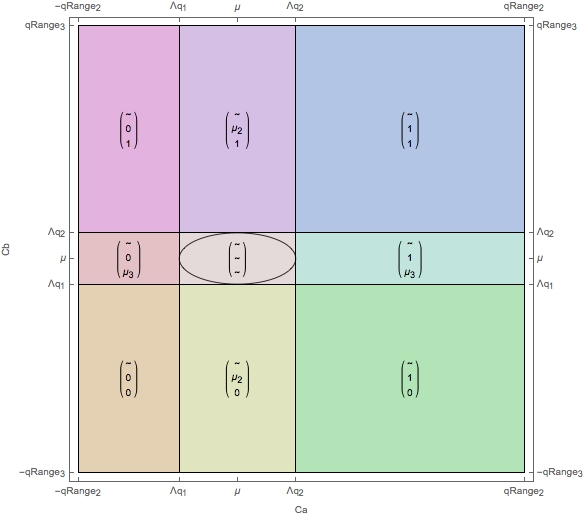
\includegraphics[width=0.80\textwidth]{Chapter4/Figs/PartitioningRegion.jpg}
      \caption{The Regions in the chromatic space. A $ \sim $ indicates values which will undergo redistribution. Regions outside the target area are allocated extreme values at the edge of the color space}  \label{fig:PartitioningRegions}
  \end{figure}
  
  
  
  \subsection{Floating the Mean}\label{sec:FloatingTheMean}
  Different lighting conditions can affect the detected pixel color. Not accounting for strongly-colored light, the affect of different lighting conditions is to increase or decrease the saturation of the color. The distribution is relatively unaffected in orientation or variance, meaning that lighting conditions can be accounted for by adjusting the mean. 
  \newcommand{\newMean}{\widetilde{\mu}}
  The algorithm adjusts to ambient lighting by first taking a reference image centered on a patch of skin and finding the mean in the LCaCb color space. This new mean $\newMean$ is then used in the current instance of the algorithm. It is adventitious to keep the mean adjustable in the routine, so this is implemented by introducing an adjustment parameter $\delta\mu$ to the routine, where $\newMean = \mu + \delta\mu$. The algorithm assumes that the adjustment is small enough that the distribution function retains the same shape aside from a translation along the axis. This allows the distribution parameters to be adjusted by simply shifting them by $\delta\mu$. 
  
  \begin{equation}
  \begin{aligned}
   \widetilde{\lambda}_1 & = \lambda_1 + \delta\mu &  \widetilde{\lambda}_2 & = \lambda_2 + \delta\mu \\
   \widetilde{\omega}_1 & = \omega_1 + \delta\mu &  \widetilde{\omega}_2 & = \omega_2 + \delta\mu 
  \end{aligned} \quad \text{Where} \quad \lambda_1 < \delta\mu < 1 - \lambda_2
  \end{equation}
  
  \subsection{Loosened Deviation}\label{sec:LoosenedDeviation}
  
 \afterpage{ \begin{figure}[h!]
    \centering
      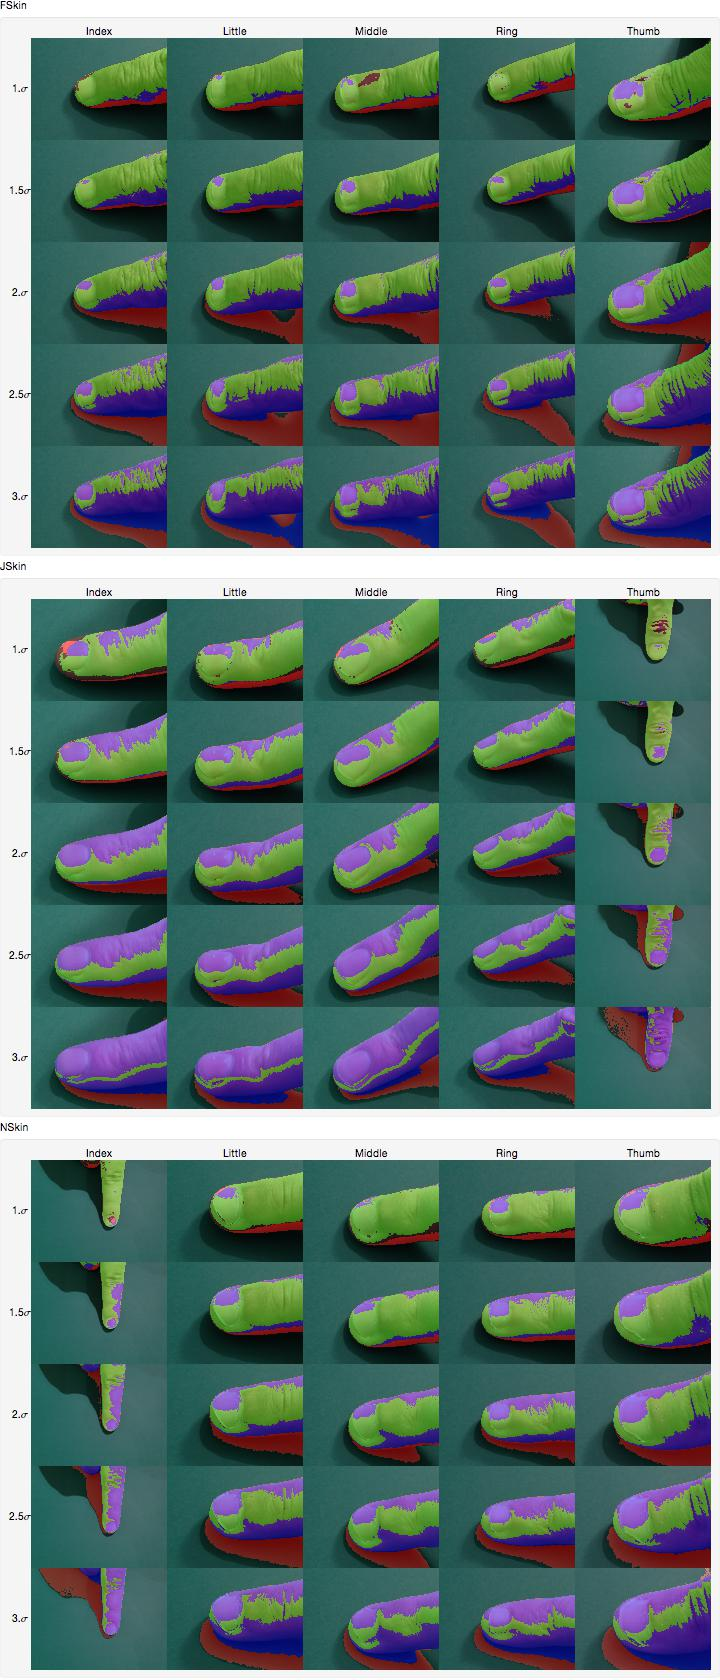
\includegraphics[width=0.85\textwidth,height = \textheight]{Chapter4/Figs/RelaxingSigma.jpg}
      \caption{A selection of images classified using the quaternary method outlined in Section \ref{sec:QuaternaryPixelClassification}, with various values of $\sigma$. It can be seen that $1\sigma$ correctly classifies the majority of pixels, however it classifies some on-digit pixels as "probably not skin", and even "not skin". $3\sigma$, meanwhile, includes large portions of shadow as "probably skin". A compromise of $2\sigma$-$2.5\sigma$ is therefore suggested.} \label{fig:RelaxedSigma}
  \end{figure}
  \clearpage
  }
  
  The standard deviation found in Chapter 3 is a very tight fit to the chromatic values taken under controlled lighting conditions. For our practical implementation, this tight fit needs to be relaxed. This is done empirically by trying out multipliers of the standard deviation $\sigma$ on the image sets. What is desired is a multiplier which relaxes the redistribution such that all the pixel values on a given digit are classified as skin, and all the background is classified as not skin. This is done empirically using the quaternary classification presented in Section \ref{sec:QuaternaryPixelClassification} below, which accounts for white-out and black-out and classifies the pixel value as "definitely skin", "probably skin", "probably not skin", and "not skin".
  
  Using a value of 2.3 times the original $\sigma$ correctly classifies the pixel values; this was found by observing tables of images similar to those in Figure \ref{fig:RelaxedSigma}. 
  
  
  \subsection{The Color Space Algorithm as Implemented}\label{sec:ColorSpaceAlgorithmAsImplemented}
  Here we present the color space algorithm in a way which most closely resembles the C++ code. The construction of the color space object is described at the end of Chapter 2; here, the operation of the algorithm is described.
  
  First, we determine the form of the distribution function for a working type $tRange$ with the source range $srcRange=2^n$  and destination range $dstRange=2^m$ expressed in terms of their bit depths.
  
  \begin{gather*}
  \begin{aligned}
  K & =  2^{m-n}  \quad & \quad  
  \tRange(\theta,\mu,\sigma)   & =  \mathbf{l} \; 2^n \quad & \quad
  \mathbf{l}  & = \min\left\{ 2^{m-n}\delta(\mu,\sigma) \right. ,  \left. \mathbf{L}(\theta) \right\} 
   \end{aligned} \\
   \begin{aligned}
    \tMin(\theta,\mu,\sigma)   & =
   \begin{pmatrix}
      0 \\
    -\mathbf{l}_2 \; 2^{n-1}  \\  
    -\mathbf{l}_3 \; 2^{n-1} \\  
   \end{pmatrix} \quad & \quad
    \tMax(\theta,\mu,\sigma)   & =
   \begin{pmatrix}
    \mathbf{l}_1 \; 2^n  \\
    \mathbf{l}_2 \; 2^{n-1}  \\  
    \mathbf{l}_3 \; 2^{n-1} \\  
   \end{pmatrix} \quad & \quad
     \Scale &=
      \mathbf{l} \otimes
     \begin{pmatrix}
       \frac{1}{3} \\
      2^{1-n } \\
      2^{1-n }  \\
     \end{pmatrix}    \\
   \end{aligned}
  \end{gather*}
  
  Substituting into the distribution function \ref{eq:disFunction} gives us
  
  \begin{equation}
\textbf{dis}(x) =  -\frac{2^n \left(\text{erf}\left(\frac{2 \mu +1}{2 \sqrt{2} \sigma }\right)+\text{erf}\left(\frac{2^{1-2 n} x-\mu }{\sqrt{2} \sigma }\right)\right)}{\text{erf}\left(\frac{2 \mu -1}{2 \sqrt{2} \sigma }\right)-\text{erf}\left(\frac{2 \mu +1}{2 \sqrt{2} \sigma }\right)} \quad \textbf{where} \quad
\begin{array}{rl}
qMin < & x  < qMax \\
0 < &\mu <1\\
0 < &\sigma <1
\end{array}
  \end{equation}
  
  This form takes the result of the rotation directly, however we wish to add the flexibility to adjust the mean and use a lookup table for the values. It is desirable to keep the lookup table as short as possible. The maximum compression of the information without losing relevant information is given by compressing to $tRange$. The number of values in the lookup table can be reduced by scaling $x$ by a range $qtRange$, which is chosen to balance lookup table size and computational scaling efficiency.  Noting that $\mathbf{l} <2$, $qRsRange$ can be chosen to be equal to $tRange$ as if $\mathbf{l} =2$, which means that $qtRange$ is a power of two, allowing the scaling to be performed by bit shifting the value of $x_{qt} = x \ll n-2$. However, in the region where the function is applied, the information is preserved at best 2-to-1, so the information density can be reduced by half $x_{qt} = x \ll n-1$. Adjusting the mean changes the bounds on the region to be redistributed such that the form of the function does not change. For this reason, we also define $x$ relative to the bounds, which allows the same lookup table to be used regardless of any adjustment to the mean.
  
    \begin{equation}
  \textbf{dis}(x) =  \begin{cases}
    \textbf{disLU}((x-\Lambda_{1}) qtRange)  & \Lambda_{1} < x < \Omega_{pq1} \\
  \textbf{disLU}((x-\Omega_{pq2}) qtRange)  & \Omega_{pq2} < x < \Lambda_{q2} \\
  \textbf{dis}(x)  & \text{Otherwise}
    \end{cases} \quad \text{where} \quad 
    qtRange = \left(\begin{smallmatrix}
    \cdots \\ 2^{1-n}\\2^{1-n}
    \end{smallmatrix}\right)
    \end{equation}
  
  Aside from these refinements, the algorithm presented in Chapter 2 is used to perform the rotation and redistribution as described. The algorithm proceeds as follows:
  
  \begin{itemize}
  \item Interactively find an adjustment to the mean  $\delta\mu$.
  \item Set the new distribution parameters.
  \item Rotate the pixel value with the $\qR$ matrix: $ pxl_{q} = \qR \cdot pxl_{RGB}$ then $ \frac{- qRsRange}{2} < pxl_{q} < \frac{ qRsRange}{2}$
  \item Partition the rotated values to avoid unnecessary processing of irrelevant information.
  \item Apply any user supplied per-pixel functions to the rotated value and add as extra channels.
  \item Redistribute the rotated values into the destination type.
  \item Apply and user supplied per-pixel functions to the redistributed values.
  \end{itemize}

\section{Pattern Recognition Routines}\label{sec:PatternRecognitionRoutines}
In this section, pattern recognition routines which use the new color space are presented and discussed.

\subsection{Quaternary Pixel Classification}\label{sec:QuaternaryPixelClassification}

\newcommand{\WoBoBool}{\underset{\scalebox{0.5}{WoBo}}{\mathbb{L}}}
\newcommand{\ColorSquareBool}{\underset{ \scalebox{0.5}[0.5]{square} }{ \mathbb{C} } }
\newcommand{\ColorEllipseBool}{\underset{ \scalebox{0.5}[0.5]{ellipse} }{ \mathbb{C} } }

\begin{figure}[h!]
  \centering
    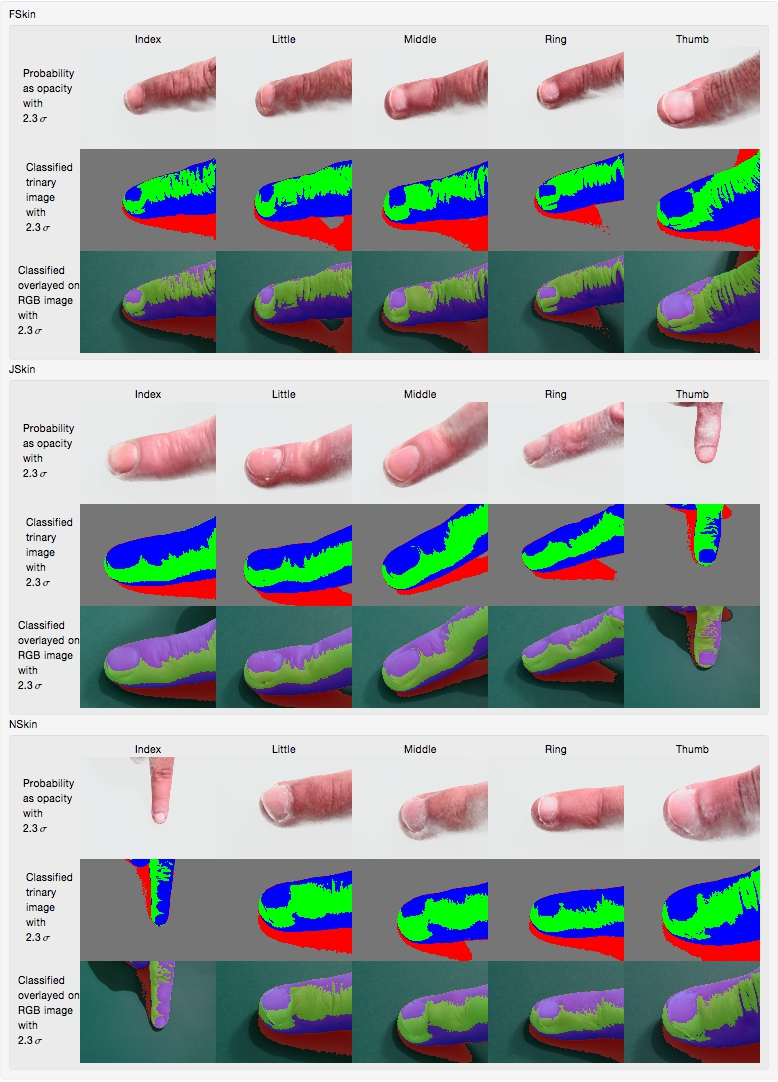
\includegraphics[width=1.0\textwidth]{Chapter4/Figs/ClassifiedSkin.jpg}
    \caption{The Quaternary Pixel Classification presented alongside the probability scored image for comparison.}\label{fig:2BitImage}
\end{figure}

We wish to classify the pixel values as either skin or not skin whist taking account of the reliability of the detected color due to whiteout and blackout effects. This is done by applying equation \ref{eq:InWoBoRegion} and setting a boolean flag $\WoBoBool$ accordingly. The square partitioning performed earlier in the algorithm also sets a boolean flag $\ColorSquareBool$ to 1 if the pixel is within the target range and to 0 otherwise. These can be combined to produce a 2-bit image which indicates both if the pixel value is in the target chromatic range and the reliability of the classification.
% 

\begin{center}
\begin{tabular}{|c|c|c|c|c|}
\hline
Correct                               & Unreliable      & \multicolumn{2}{|c|}{Image Bit} & \multicolumn{1}{|c|}{\multirow{2}{*}{Comment}}  \\ \cline{1-4}
Color $\ColorSquareBool$ & $\WoBoBool$ & $\ColorSquareBool$ & XOR($\ColorSquareBool$, $\WoBoBool$) & \\\hline
0 & 0 & 0 & 0 &  Definitely not the target \\\hline % & Wrong Color &    Reliable Luminosity 
0 & 1 & 0 & 1  & \begin{tabular}{l} Possibly the target but \\ shifted out of the target \\ chromatic region by WOBO. \end{tabular} \\\hline % & Wrong Color & Unreliable Luminosity
1 & 1 & 1 & 0  & \begin{tabular}{l} Probably the target but possibly \\ shifted into the target chromatic \\ region by WOBO \end{tabular} \\\hline % &   Right Color &    Reliable Luminosity
1 & 0 & 1 & 1  & Definitely the target \\\hline % &   Right Color & Unreliable Luminosity
\end{tabular}
\end{center}


This produces a 2-bit image, as seen in Figure \ref{fig:2BitImage}. For this purpose, a 2-bit data type was added to OpenCV. The question then is how to use it. Essentially, we have four different states: values which are neither the right color nor in the right region; values which are possibly the right color, but because they're outside the valid region, they've potentially suffered from white-out and black-out; values which are in the right region, but the wrong color, and we are certain that they are not skin; and finally, values which are in the valid region and are of the right color. In the following subsections we will present some useful methods which take advantage of this quaternary classified image.


\chapter{Shape Fitting Methods}

\section{The `Hurdle' Method}\label{sec:HurdleMethod}
The Hurdle method is an algorithm for finding a path inside an object using the quaternary classified image. The Hurdle method follows straight line paths in the object. As written, it is flexible enough to follow any straight line, however the current implementation takes a direction vector and evaluates at multiples of that direction vector. This means that non-horizontal and non-vertical lines are not guaranteed to be continuous. This is because the pixel values are not found using Bresenham's line algorithm. The algorithm has two thresholds --- a high and a low threshold. Whilst the pixel values remain in the high threshold, the path end point variable is updated; when the pixel values are in the lower threshold, the algorithm continues along the path, but without updating the path end point. This allows the path to pass through artifacts (i.e. pixel values which are inside the object but which have been misclassified), but does not allow the path to extend outside of the object into regions which are, for instance, in the shadow of the object.
 
 \section{The `Mean-Median' Method}\label{sec:MeanMedian}
 Computer vision algorithms often produce very noisy signals with significant anomalies and outliers in the data. Taking an arithmetic mean is therefore problematic as an outlier can significantly alter the mean. The Mean-Median method --- similar to the "k-Nearest Neighbors" algorithm --- solves this problem by taking a confidence interval around the median and then taking the mean of the points within this interval. This method is a useful adaptation of methods like the k-Nearest Neighbors in that it solves the outlier problem.
 
\section{The `Filament Fill' Method}\label{sec:FilamentFill}

\begin{figure}[h!]
  \centering
    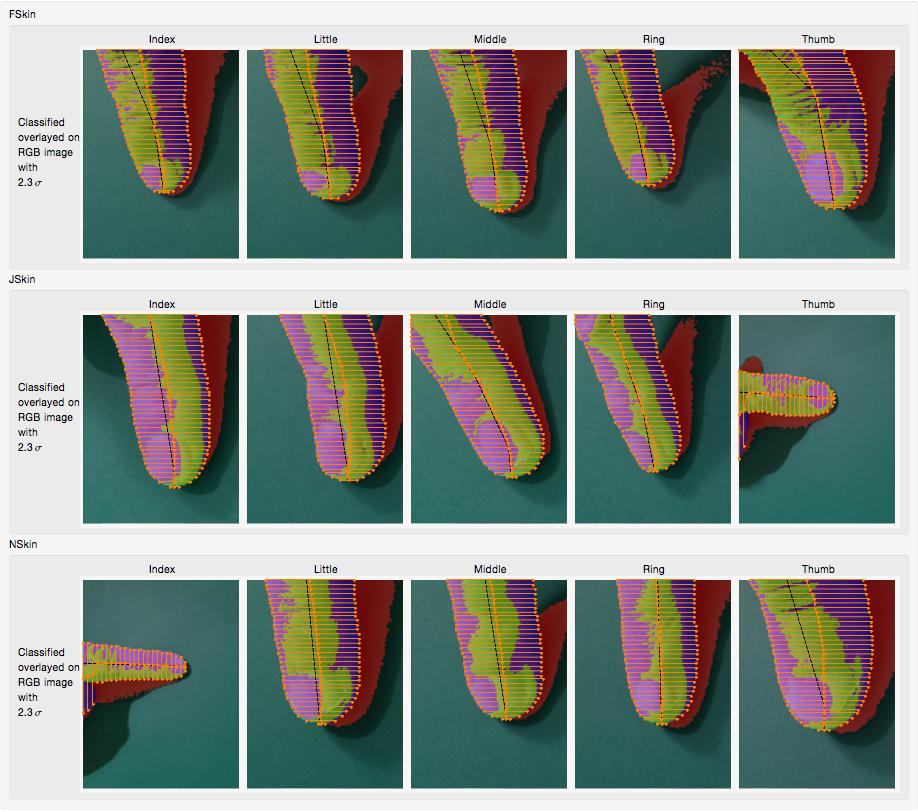
\includegraphics[width=0.95\textwidth]{Chapter4/Figs/FillamentFill.jpg}
    \caption{The 'Filament Fill' Method.}\label{fig:FillamentFill}
\end{figure}

The Filament Fill method takes a path --- given as a sequence of points --- within an object and finds the edges of the object using the Hurdle method running away from the path within the object. Assuming a horizontally-oriented object, the path's extent in the horizontal direction is divided equally into points, and these points are used to start the Hurdle method in the vertical directions, and vice versa for vertical-oriented objects.

For the purposes of the shape detection algorithms, there are metrics that are applied which suffer from noise and anomalies, where the noise is due to the natural variability of human digits from regular geometric forms, and the anomalies are due to miss-detections of the edges of the digit. We assume that the anomalous results are extreme values, however we acknowledge that the most common (mode) or middle (median) values may not be representative of the best geometric approximation for the shape. The Mean-Median method \ref{sec:MeanMedian} solves this problem for this particular application.

\section{The `Kink Fit' Method}\label{sec:KinkFitMethod}
The Kink Fit algorithm takes in a set of 2D points, where the first component is taken to be the independent variable and the second component is taken to be the dependent variable. This assumption excludes the possibility of truly vertical lines being presented to the algorithm. The Kink Fit algorithm fits a function which consists of two straight-line segments to a set of points. Unfortunately, currently the only piecewise linear fitting function is the proprietary MARS algorithm which, aside from being commercial, is overkill for this particular problem, which has a small number of points which are well-aligned. 

The Kink Fit algorithm relies on the fact that we know that the points are in order; it chooses a point and divides the set in two, and then performs a standard, least squares linear fit to the two sets. Both sets include the point at which the set is divided. 

The fit is also assumed to be continuous, except in the first derivative. The algorithm as described above may produce two lines which do not intersect between the second-to-last data point used for the first line and the second data point used for the second line. The algorithm needs to ensure that this is the case. This is achieved by shifting the second half of the data set by the end point of the linear fit to the first half of the data set. The point at which the two linear fits intersect is found, and if that point is between the second-to-last point in the first set, and a second point in the second set (i.e. the points on either side of the point of division), then the fit is considered to be acceptable. If the fit is not acceptable, it indicates that there's a discontinuity in position rather than simply being a discontinuity in the first derivative. This is handled by choosing the point on the fit to the first set closest to the intersection within the bounds of the points on either side of the point of division. The linear fit is then performed with only the gradient as the free parameter, guaranteeing that the line will have passed through this limiting point.

The algorithm then finds the residuals, and then finds the average of the square of the residuals. This is considered the score for dividing the set of points at that position. The algorithm finds the point which minimizes the score using a bisecting algorithm; if a linear fit to the data has a low score, then the Kink Fit algorithm is considered unnecessary and the digit is assumed to be in a relaxed, straight, neutral pose. The algorithm specifies a minimum number of points to be included in a set, as this avoids the problem of dividing into sets which contain only one point.

%\begin{figure}[h!]
%  \centering
%    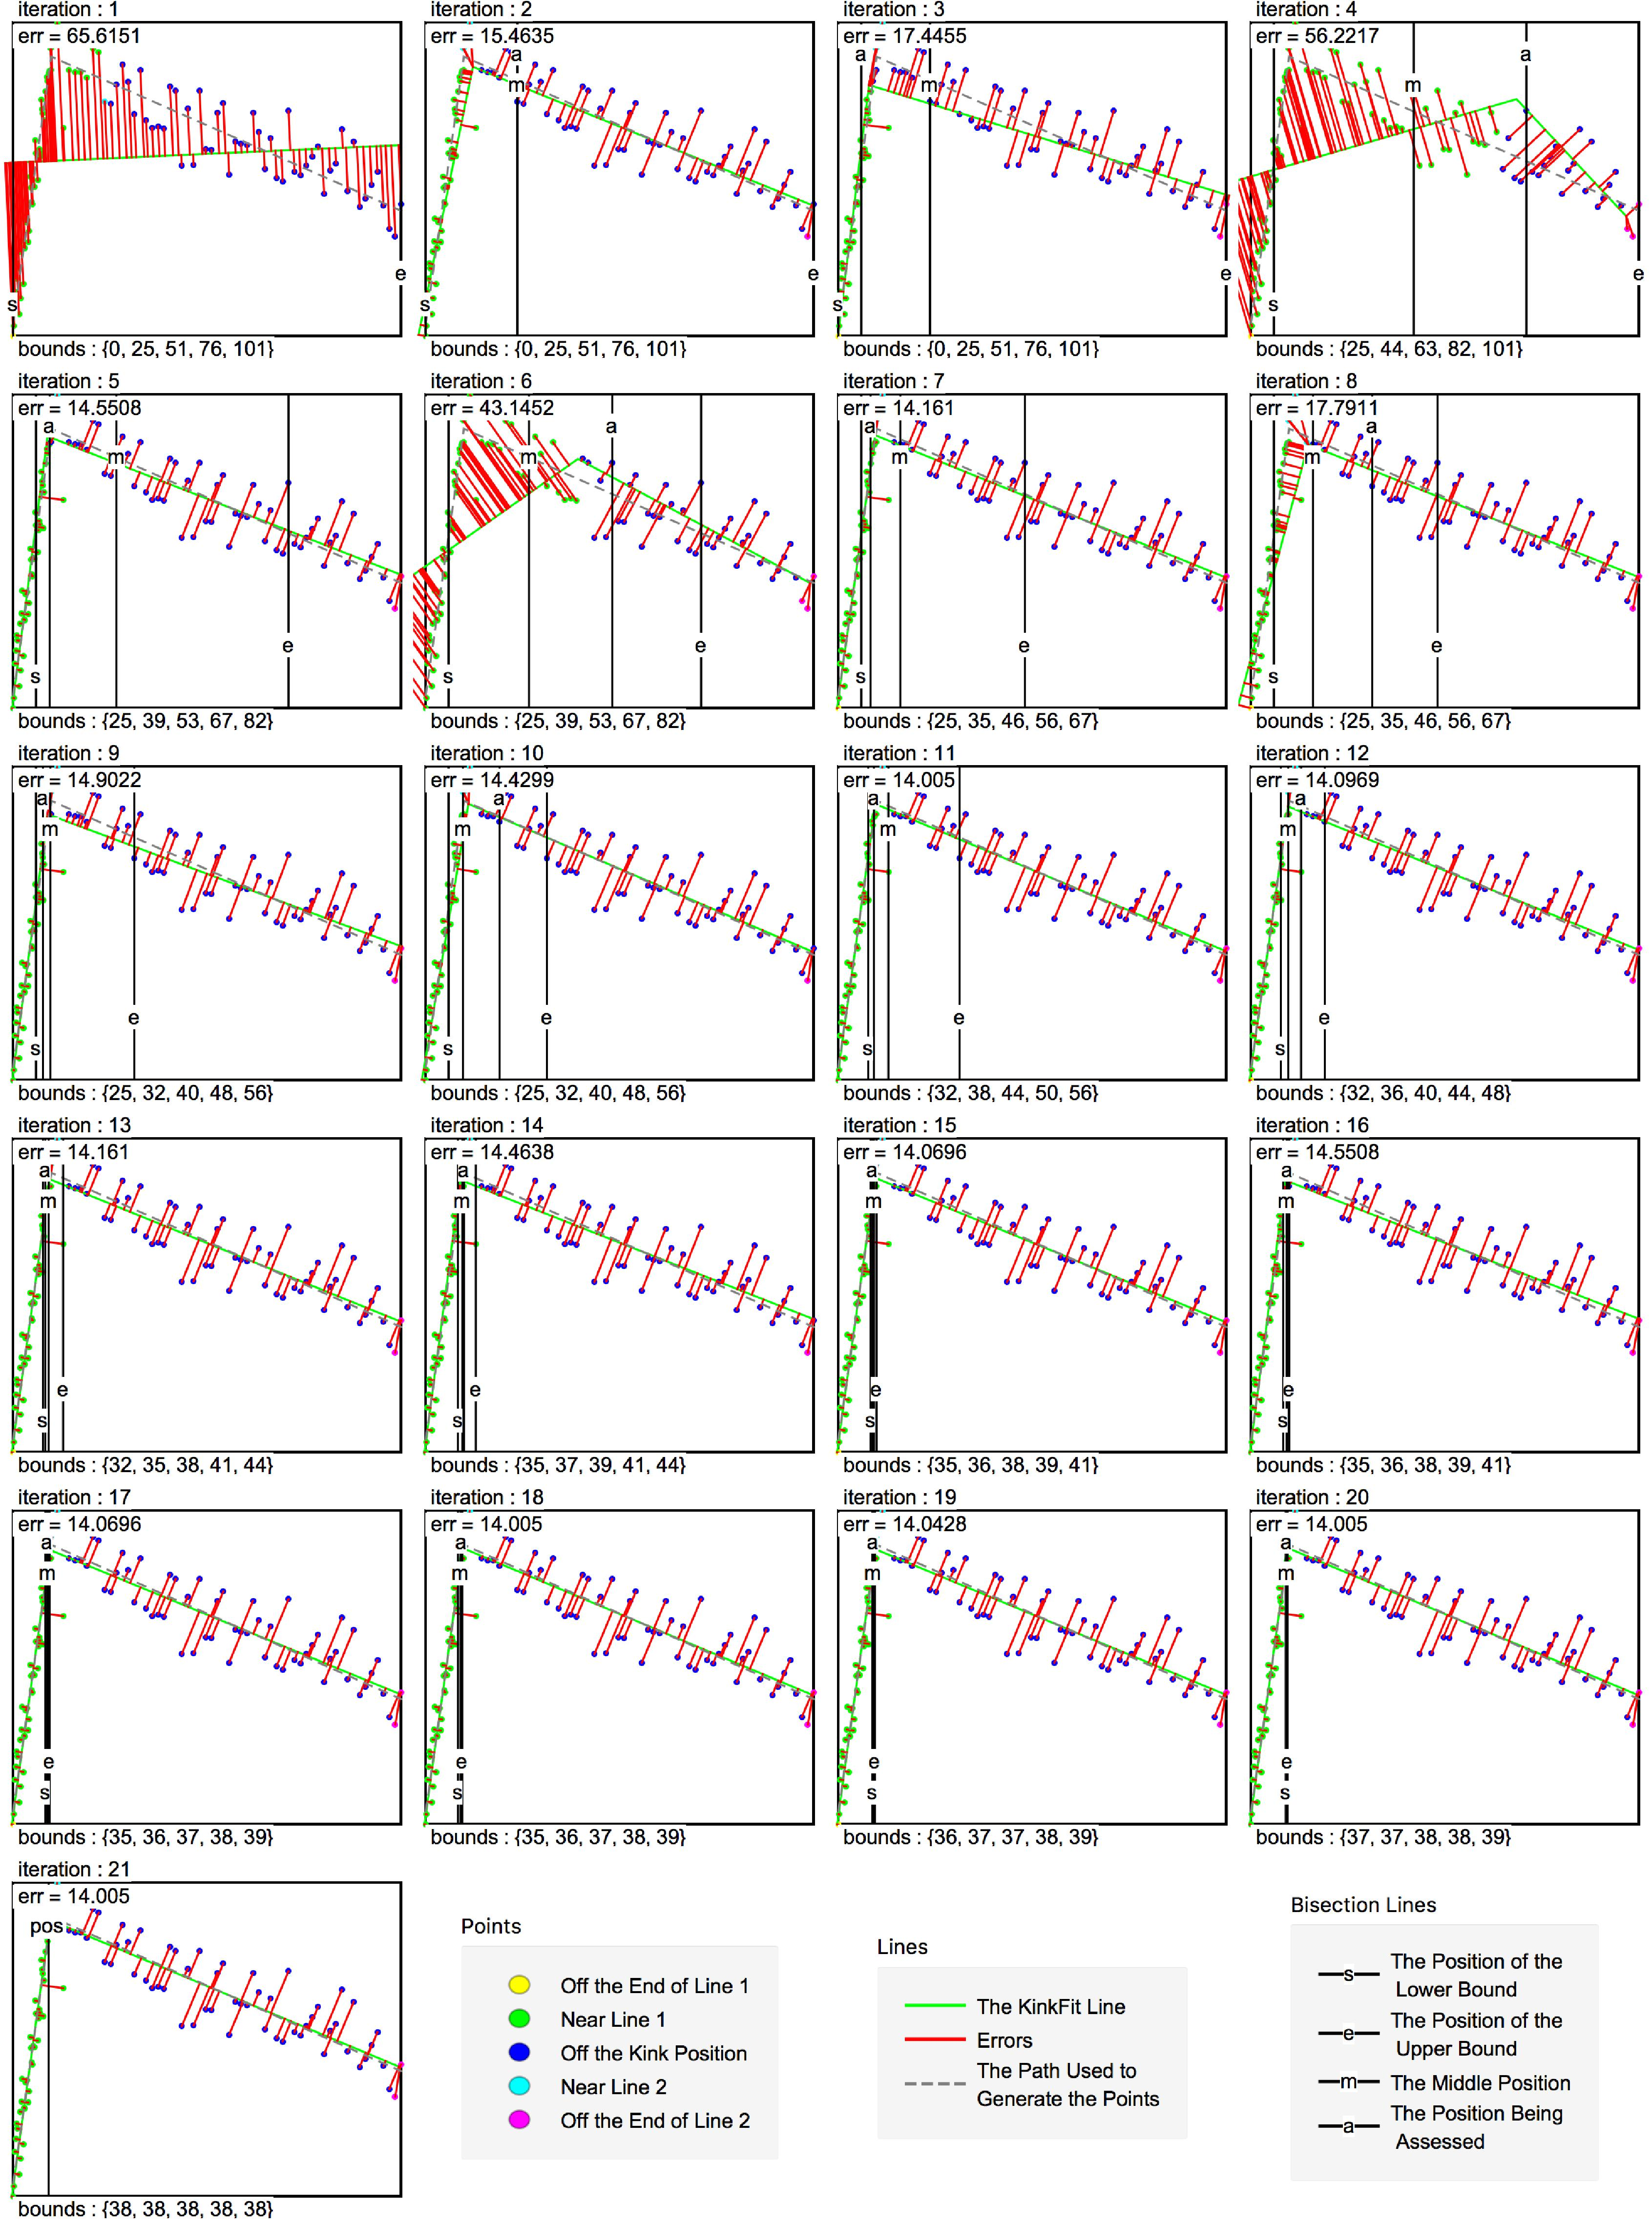
\includegraphics[width=0.92\textwidth]{Chapter4/Figs/KinkFit_A.jpg}
%    \caption{KinkFitA}\label{fig:KinkFitA}
%\end{figure}

%\begin{figure}[h!]
%  \centering
%    \includegraphics[width=0.95\textwidth]{Chapter4/Figs/KinkFit_B.jpg}
%    \caption{KinkFitB}\label{fig:KinkFitB}
%\end{figure}

\begin{figure}[h!]
  \centering
    \includegraphics[width=0.88\textwidth]{Chapter4/Figs/KinkFit_C.jpg}
    \caption{Example A of the KinkFit algorithm in action, showcasing its reliability over several iterations.}\label{fig:KinkFitC}
\end{figure}

%\begin{figure}[h!]
%  \centering
%    \includegraphics[width=0.85\textwidth]{Chapter4/Figs/KinkFit_D.jpg}
%    \caption{KinkFitD}\label{fig:KinkFitD}
%\end{figure}

%\begin{figure}[h!]
%  \centering
%    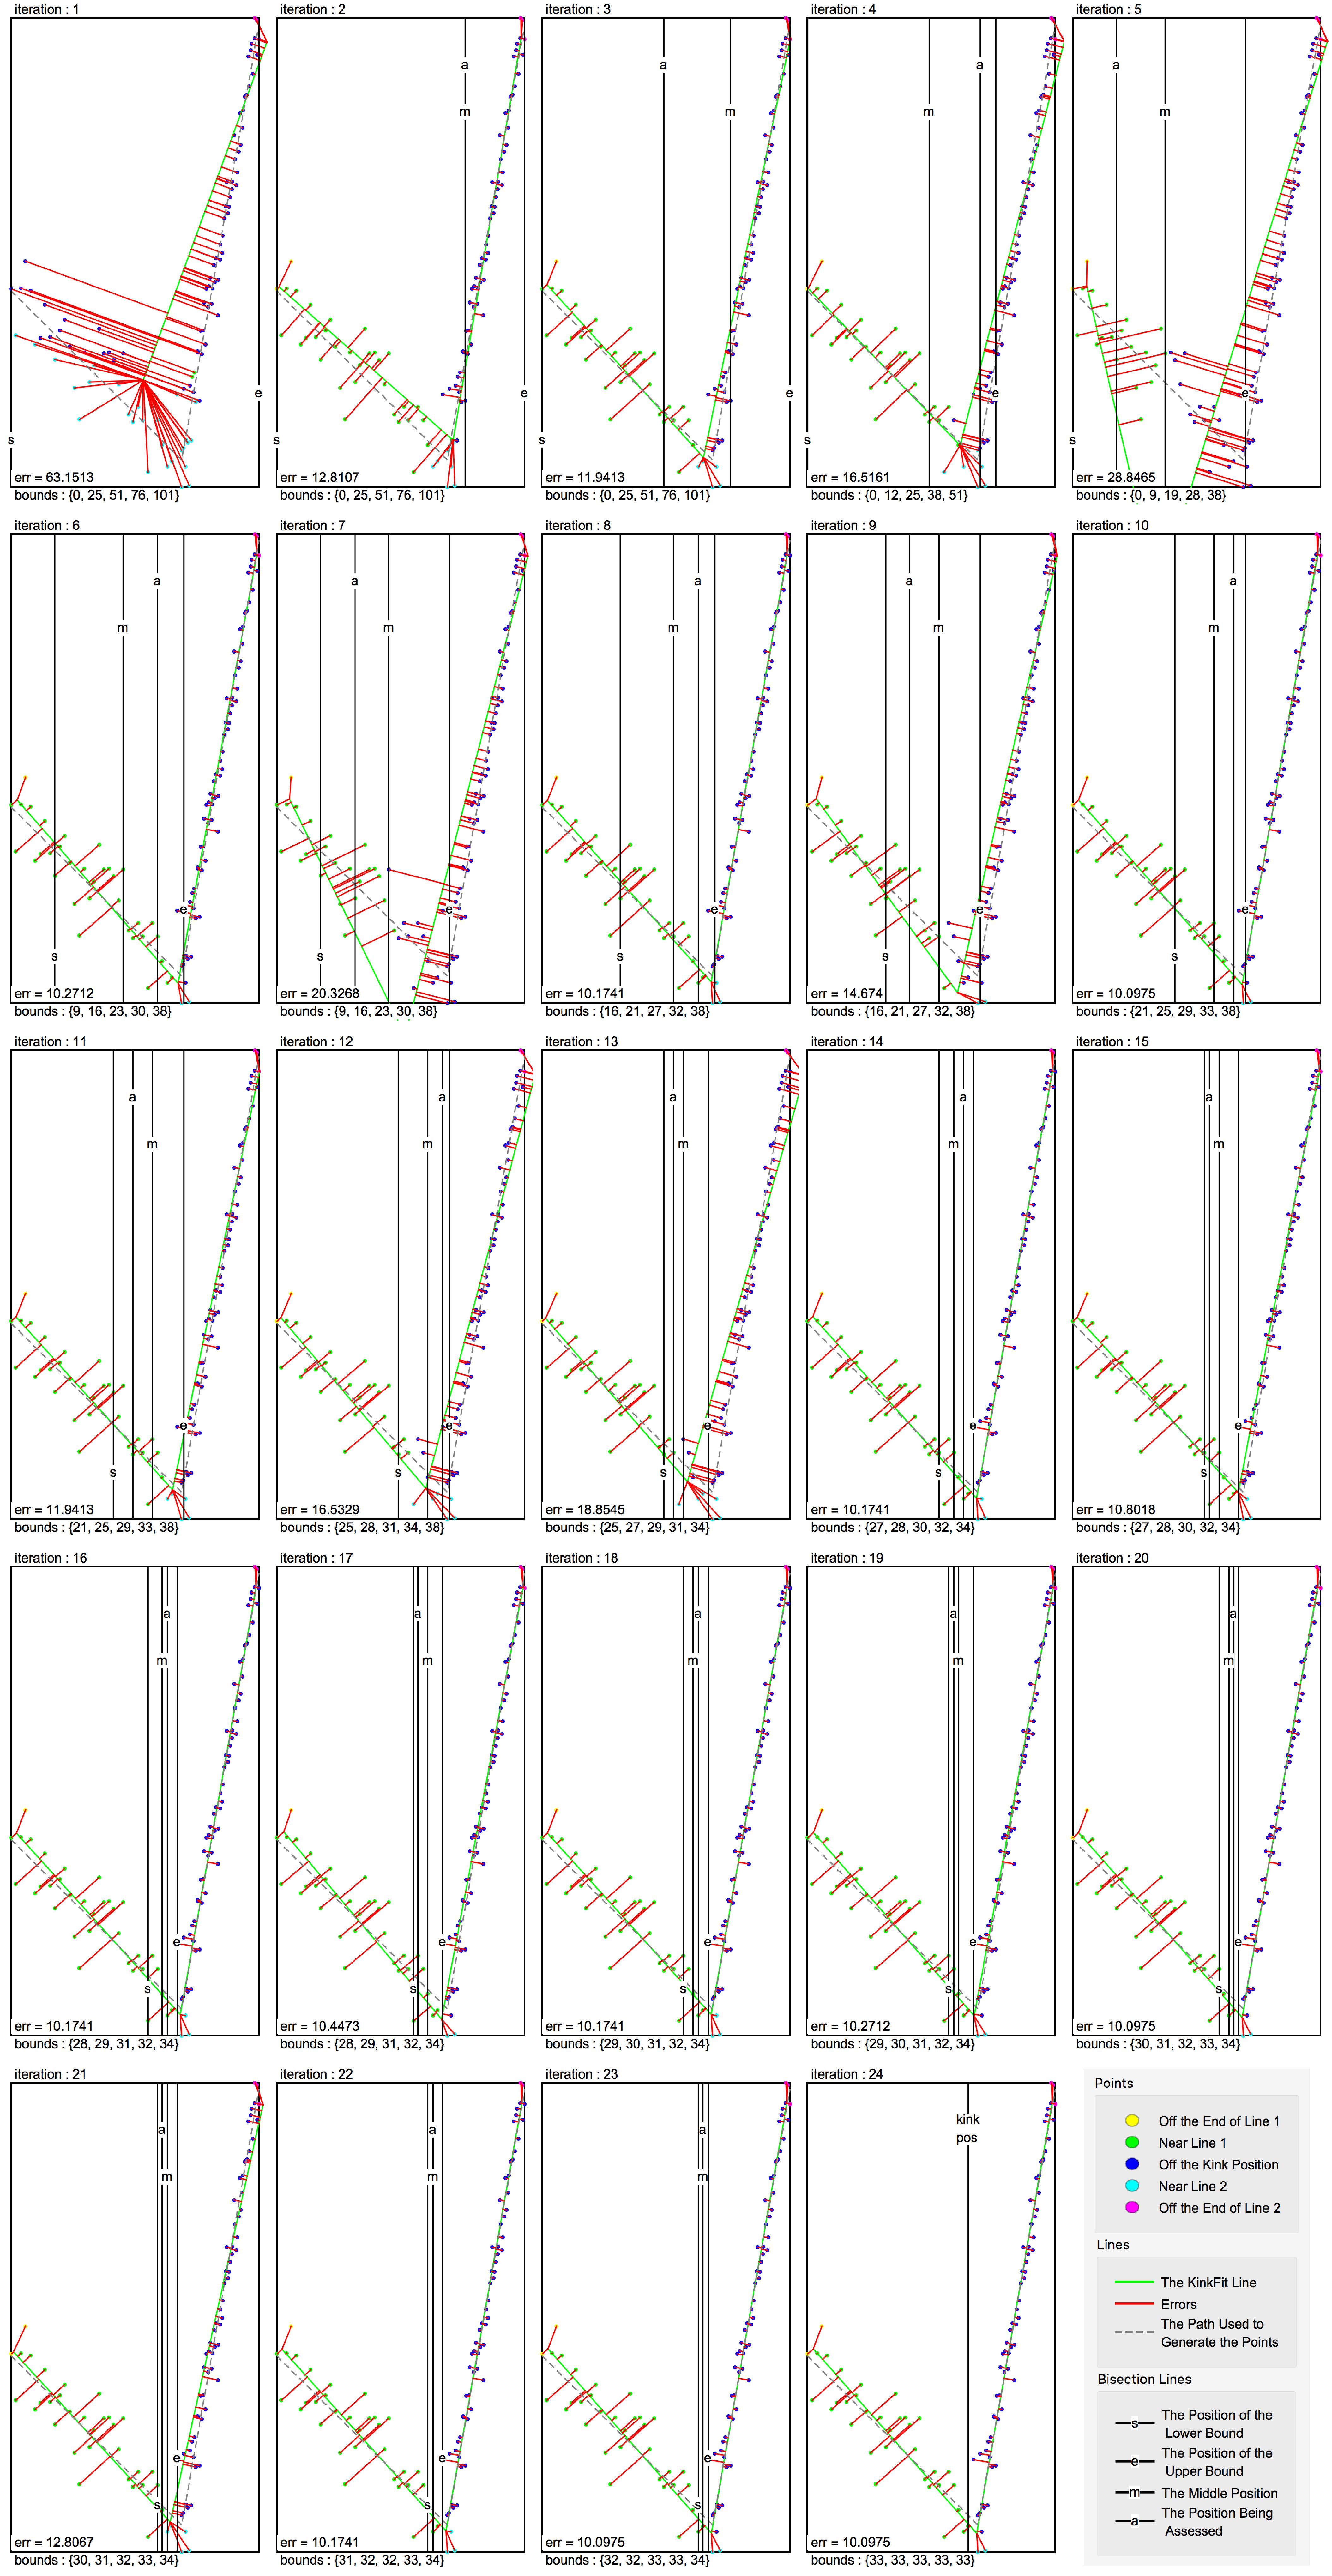
\includegraphics[width=0.80\textwidth]{Chapter4/Figs/KinkFit_E.jpg}
%    \caption{KinkFitE}\label{fig:KinkFitE}
%\end{figure}

\begin{figure}[h!]
  \centering
    \includegraphics[width=0.95\textwidth]{Chapter4/Figs/KinkFit_F.jpg}
    \caption{Example B of the KinkFit algorithm in action, showcasing its reliability over several iterations.}\label{fig:KinkFitF}
\end{figure}

%\begin{figure}[h!]
%  \centering
%    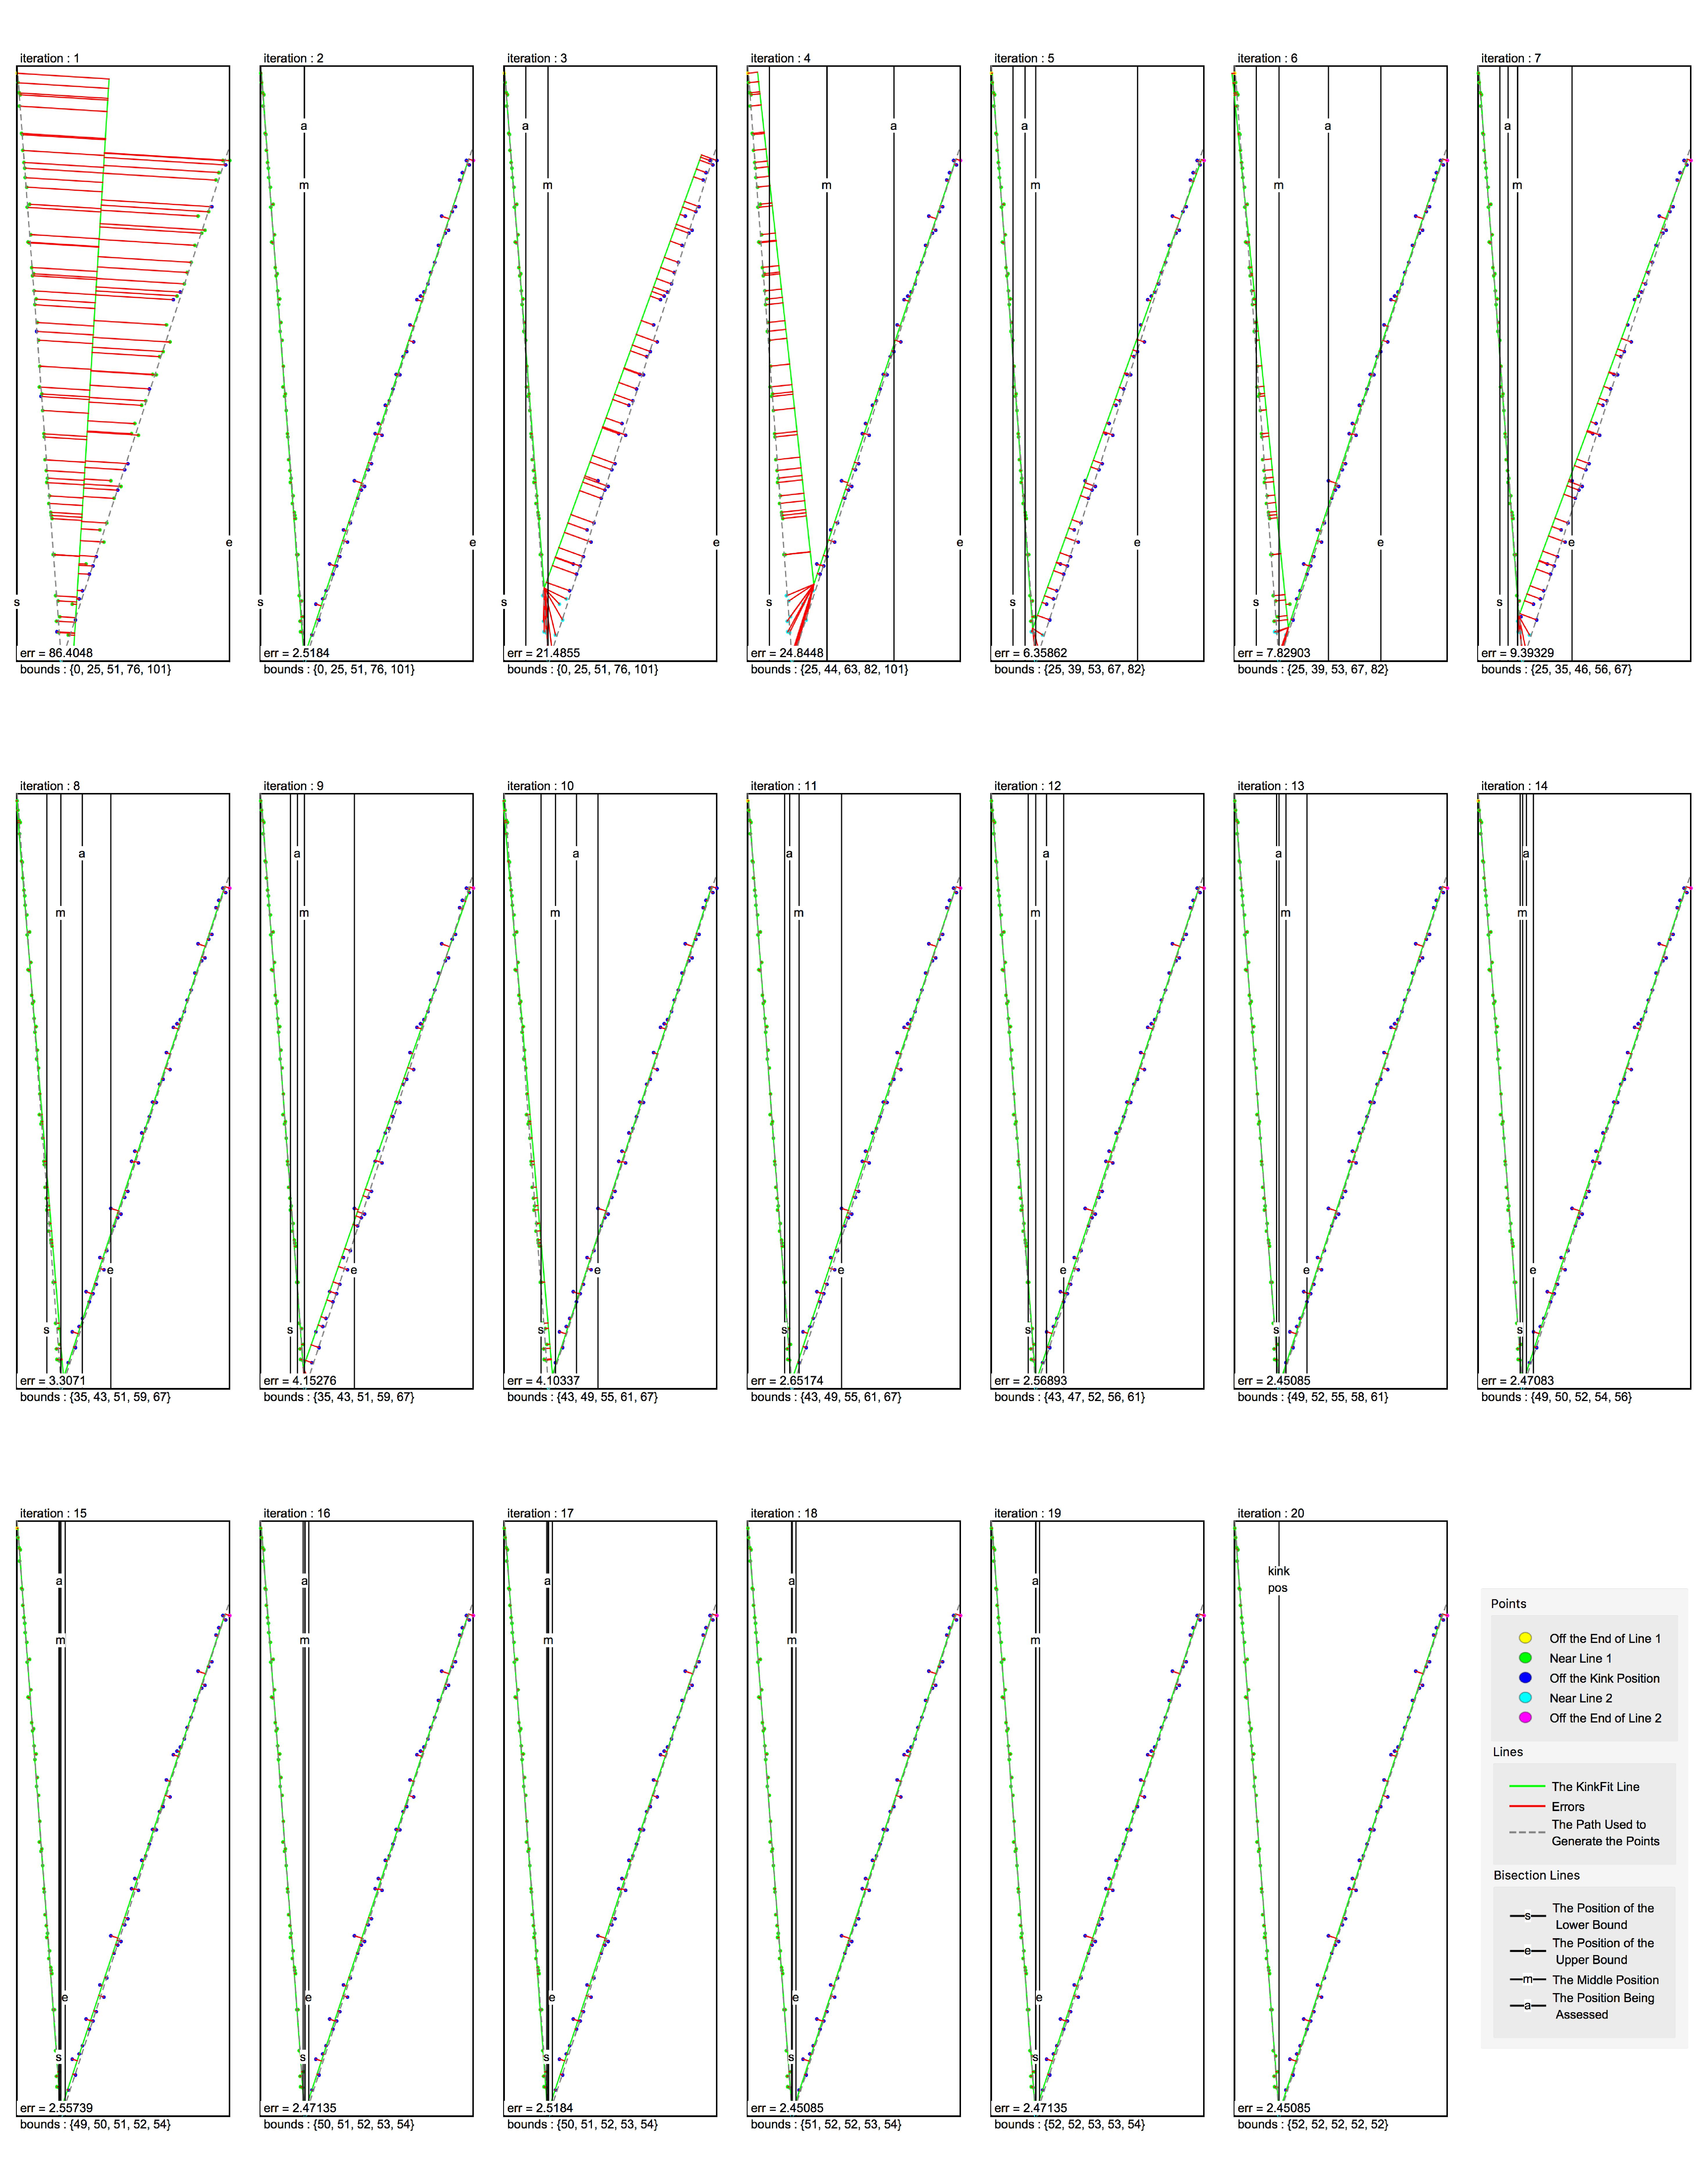
\includegraphics[width=0.95\textwidth]{Chapter4/Figs/KinkFit_G.jpg}
%    \caption{KinkFitG}\label{fig:KinkFitG}
%\end{figure}

\begin{figure}[h!]
  \centering
    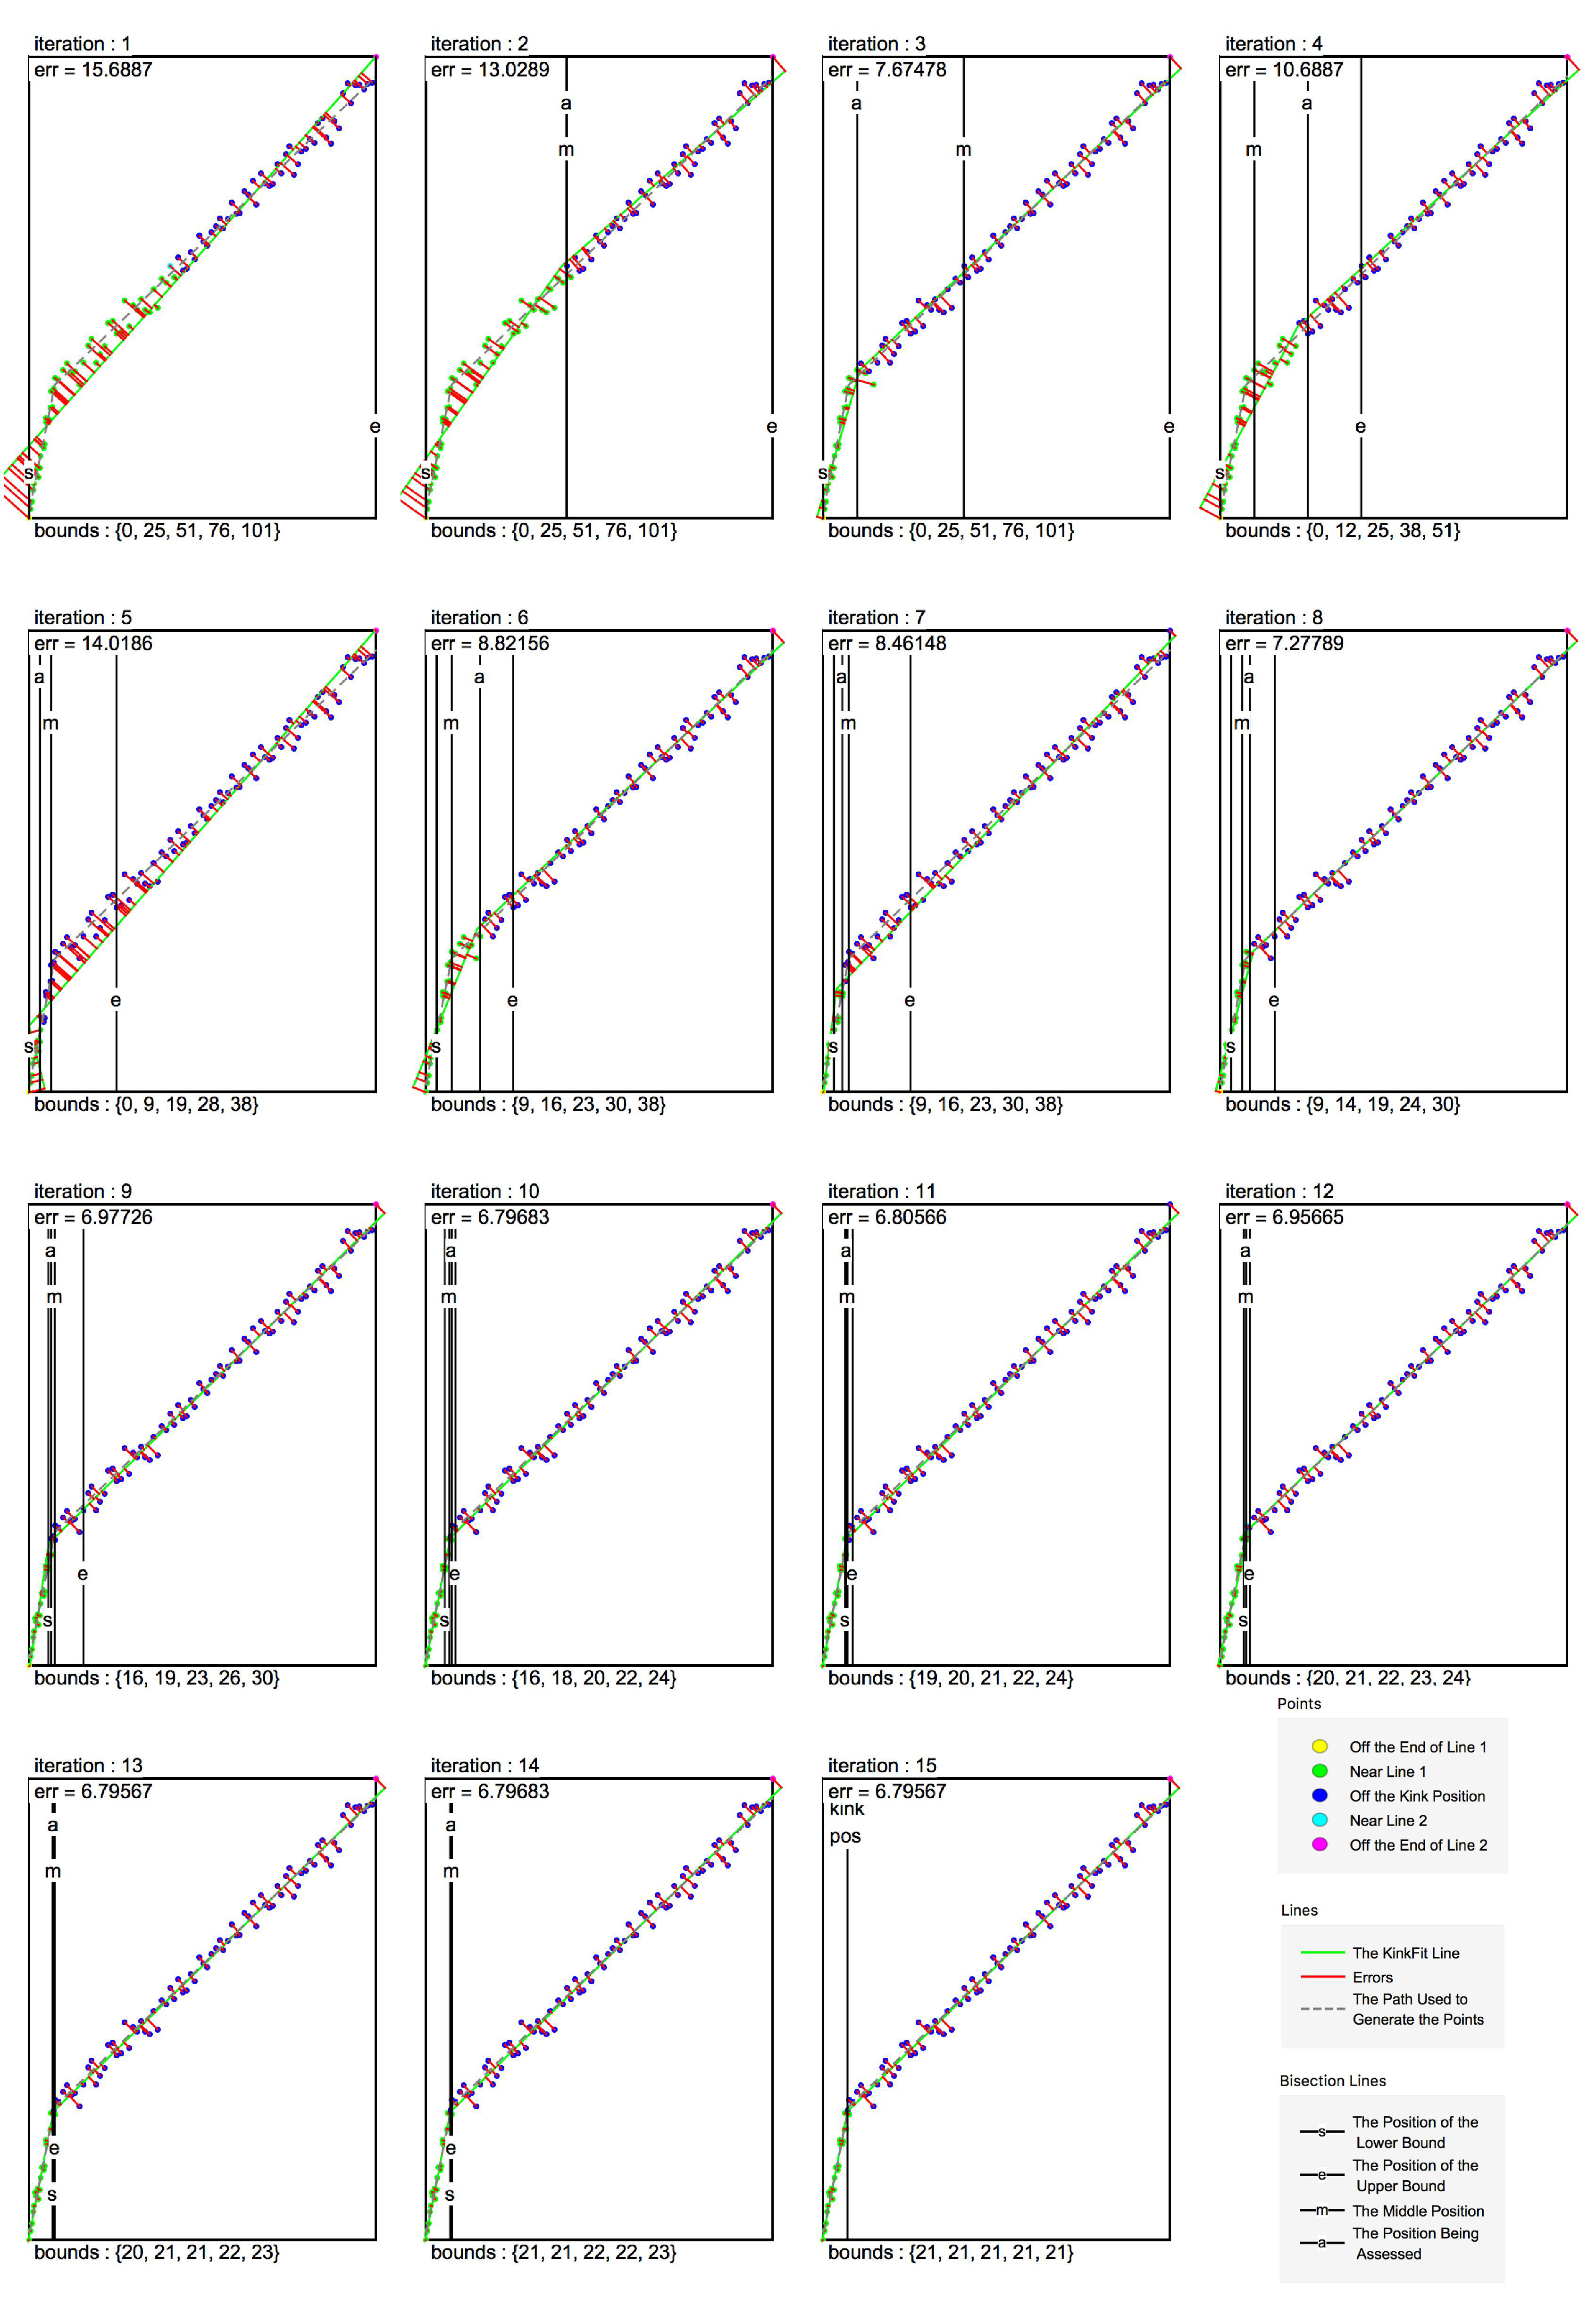
\includegraphics[width=0.95\textwidth]{Chapter4/Figs/KinkFit_H.jpg}
    \caption{Example C of the KinkFit algorithm in action, showcasing its reliability over several iterations.}\label{fig:KinkFitH}
\end{figure}

%\begin{figure}[h!]
%  \centering
%    \includegraphics[width=0.95\textwidth]{Chapter4/Figs/KinkFit_I.jpg}
%    \caption{KinkFitI}\label{fig:KinkFitI}
%\end{figure}

%\begin{figure}[h!]
%  \centering
%    \includegraphics[width=0.95\textwidth]{Chapter4/Figs/KinkFit_J.jpg}
%    \caption{KinkFitJ}\label{fig:KinkFitJ}
%\end{figure}

\begin{figure}[h!]
  \centering
    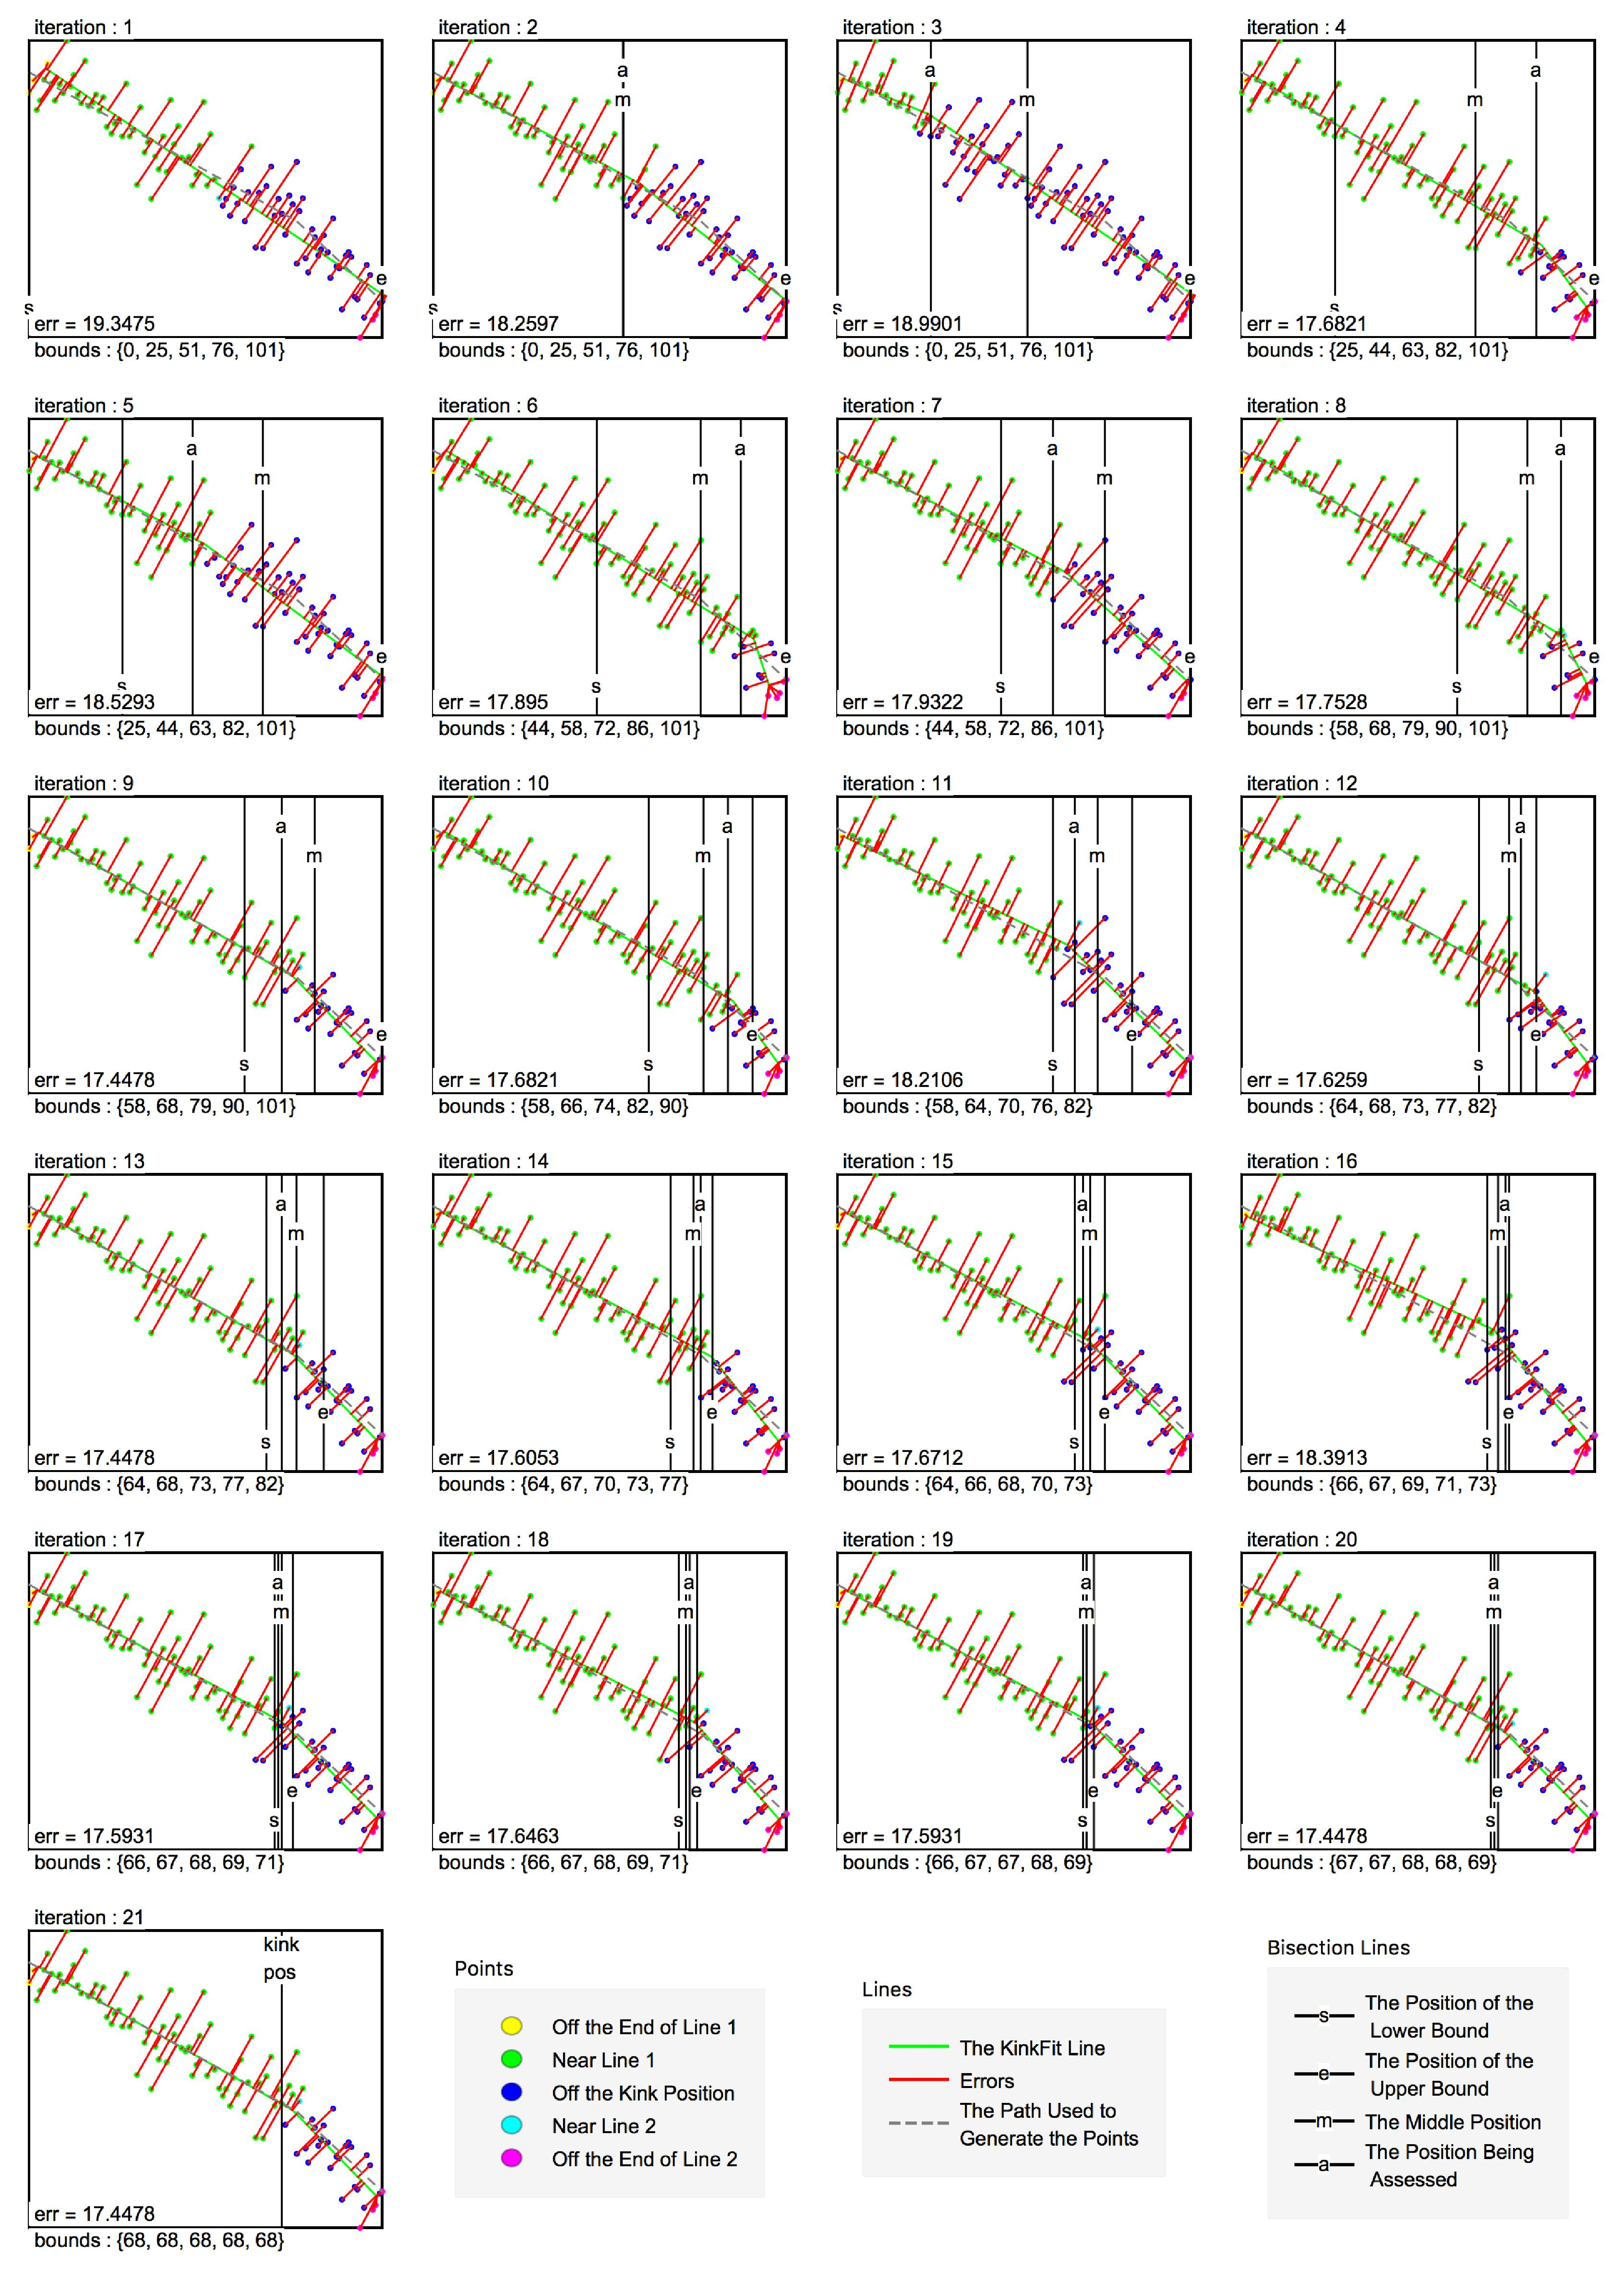
\includegraphics[width=0.95\textwidth]{Chapter4/Figs/KinkFit_K.jpg}
    \caption{Example D of the KinkFit algorithm in action, showcasing its reliability over several iterations.}\label{fig:KinkFitK}
\end{figure}

%\begin{figure}[h!]
%  \centering
%   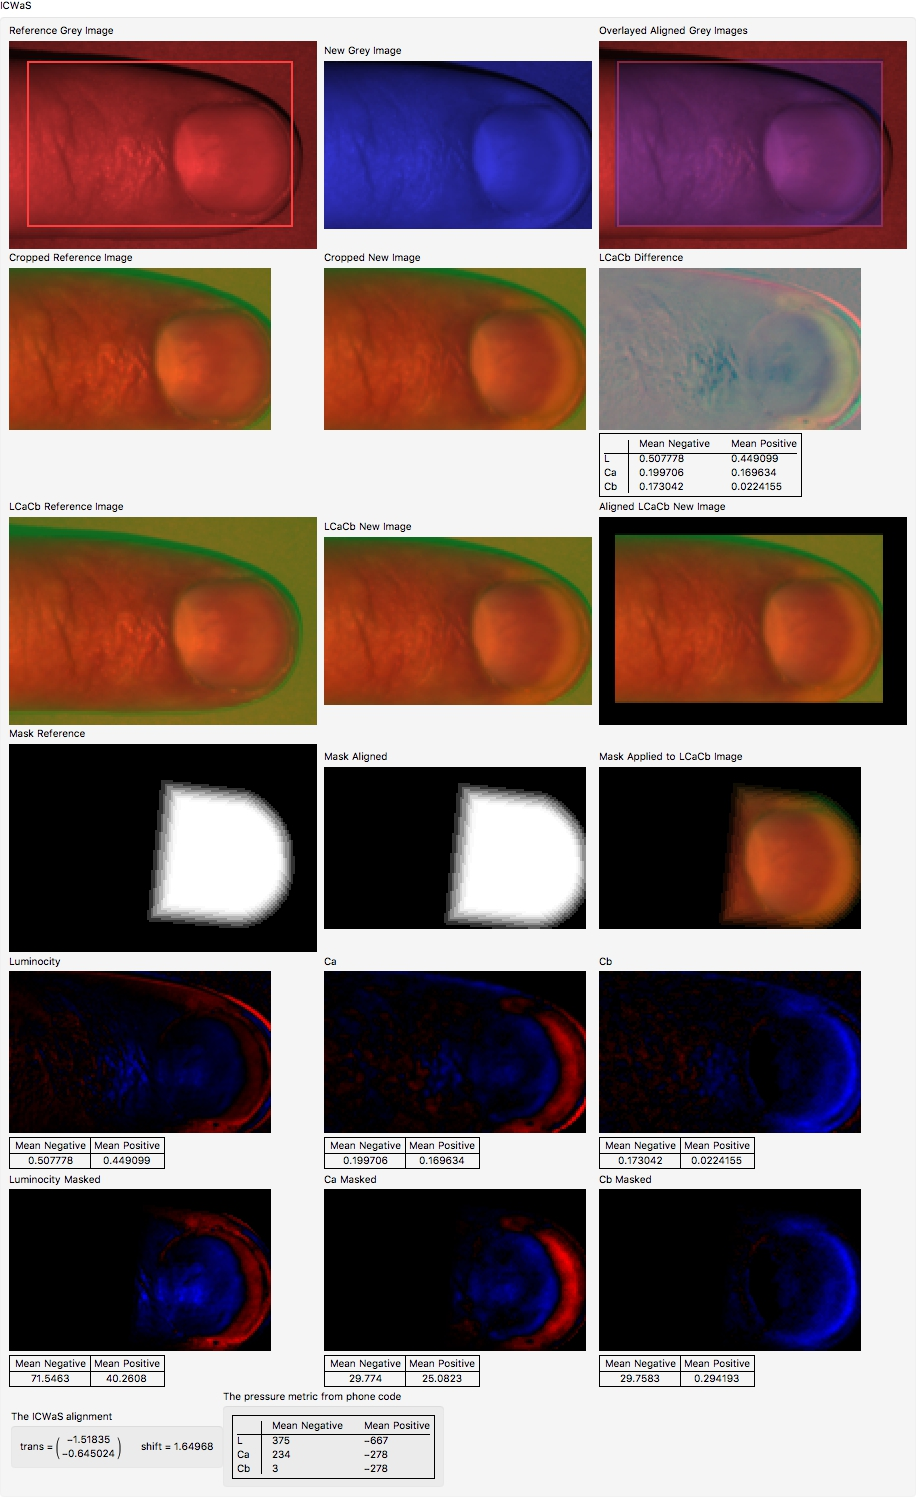
\includegraphics[width=0.95\textwidth]{Chapter4/Figs/ICWaS1.jpg}
%    \caption{ICWaS1}\label{fig:ICWaS1}
%\end{figure}
%\begin{figure}[h!]
%  \centering
%    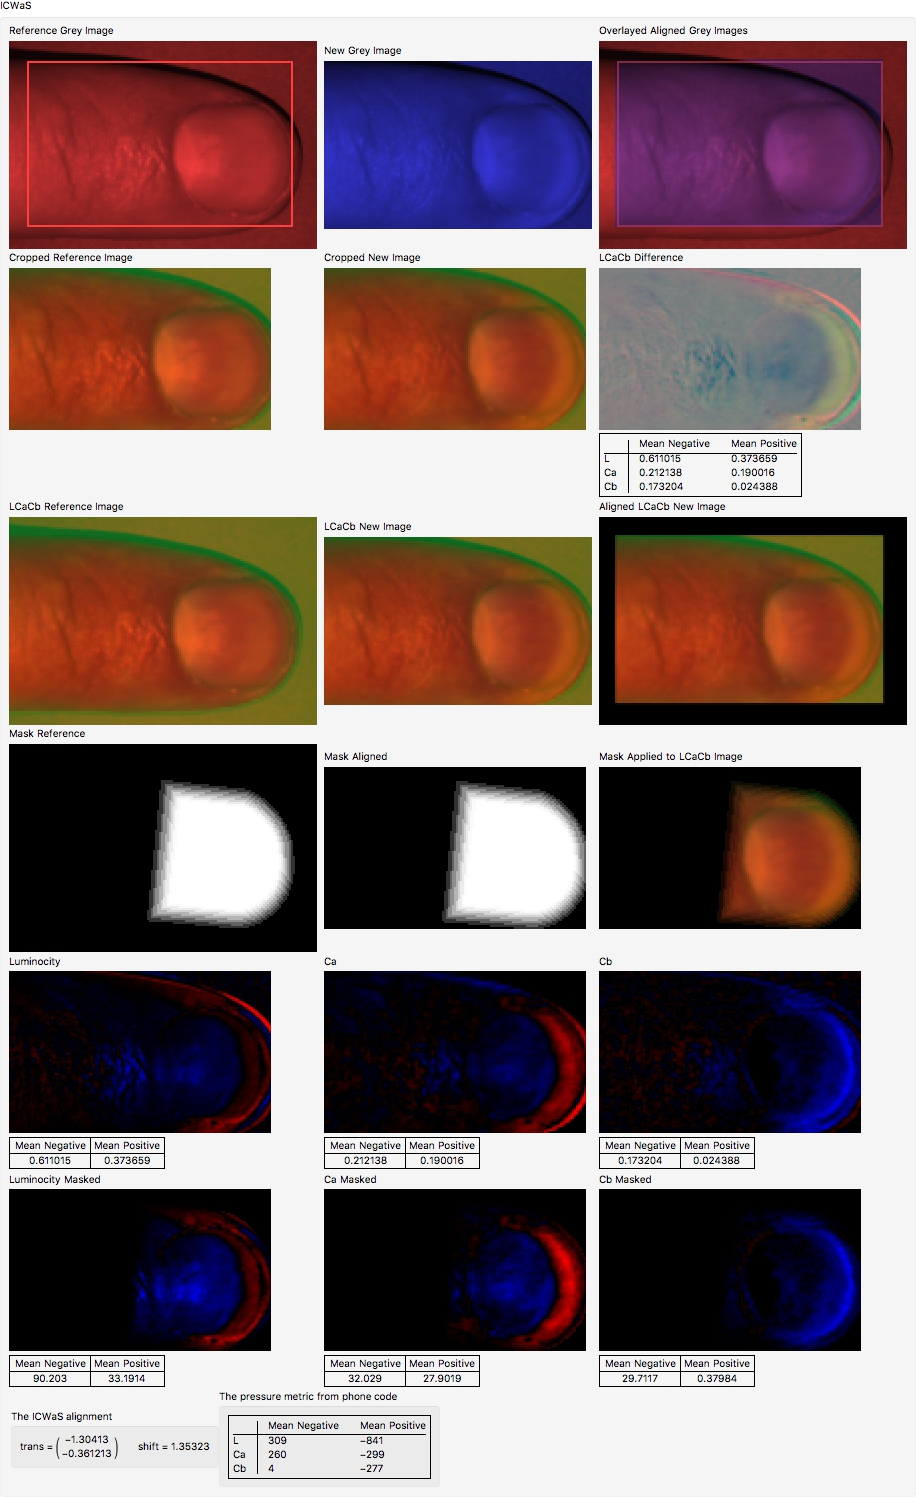
\includegraphics[width=0.95\textwidth]{Chapter4/Figs/ICWaS2.jpg}
%    \caption{ICWaS2}\label{fig:ICWaS2}
%\end{figure}
%\begin{figure}[h!]
%  \centering
%    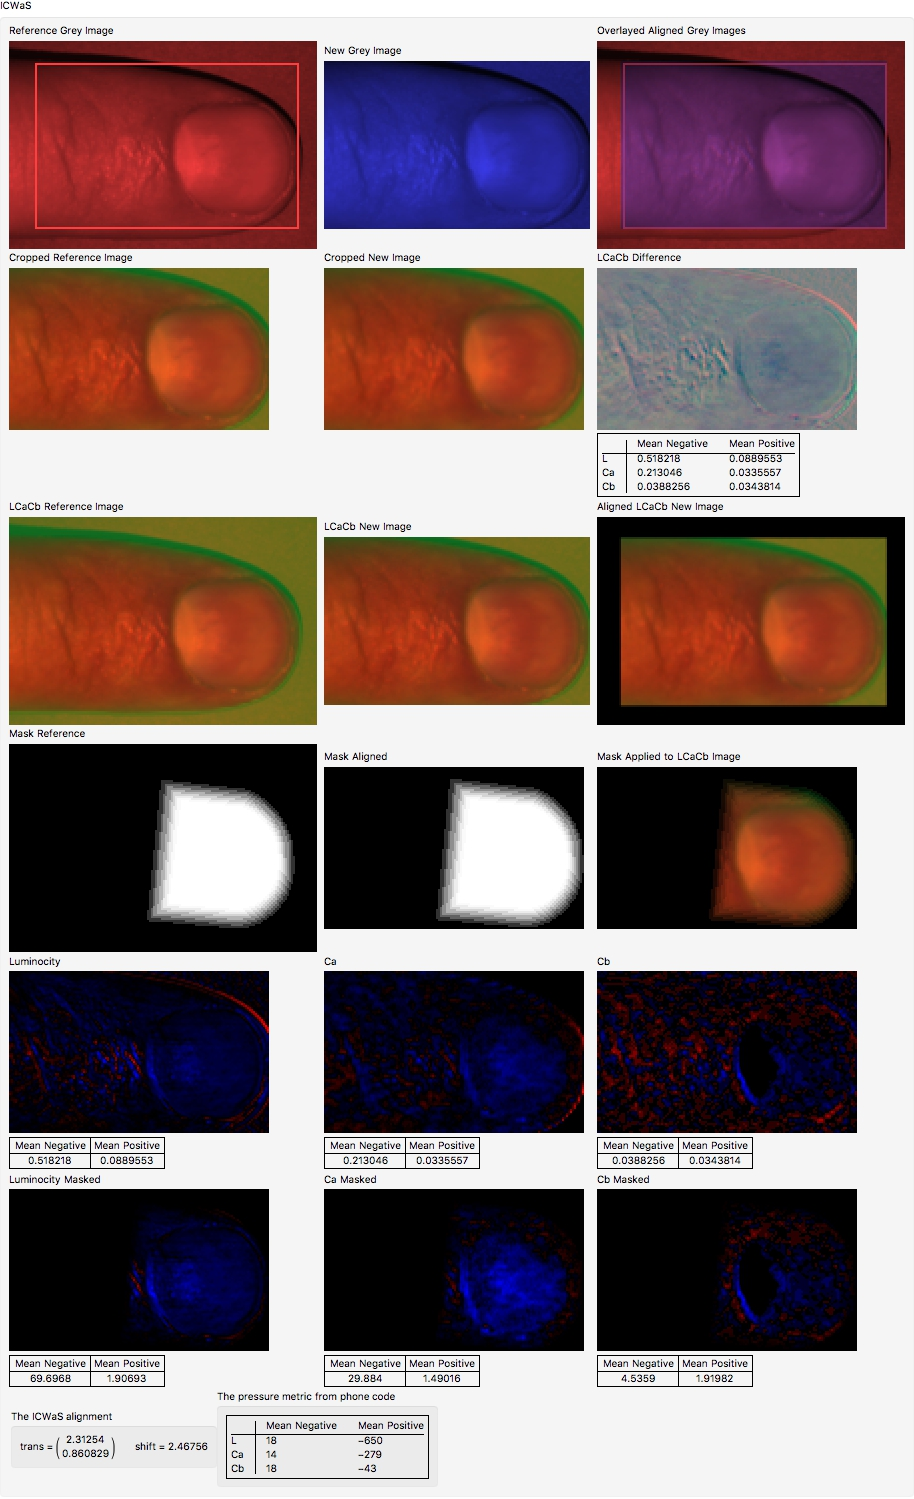
\includegraphics[width=0.95\textwidth]{Chapter4/Figs/ICWaS3.jpg}
%    \caption{ICWaS3}\label{fig:ICWaS3}
%\end{figure}
%\begin{figure}[h!]
%  \centering
%    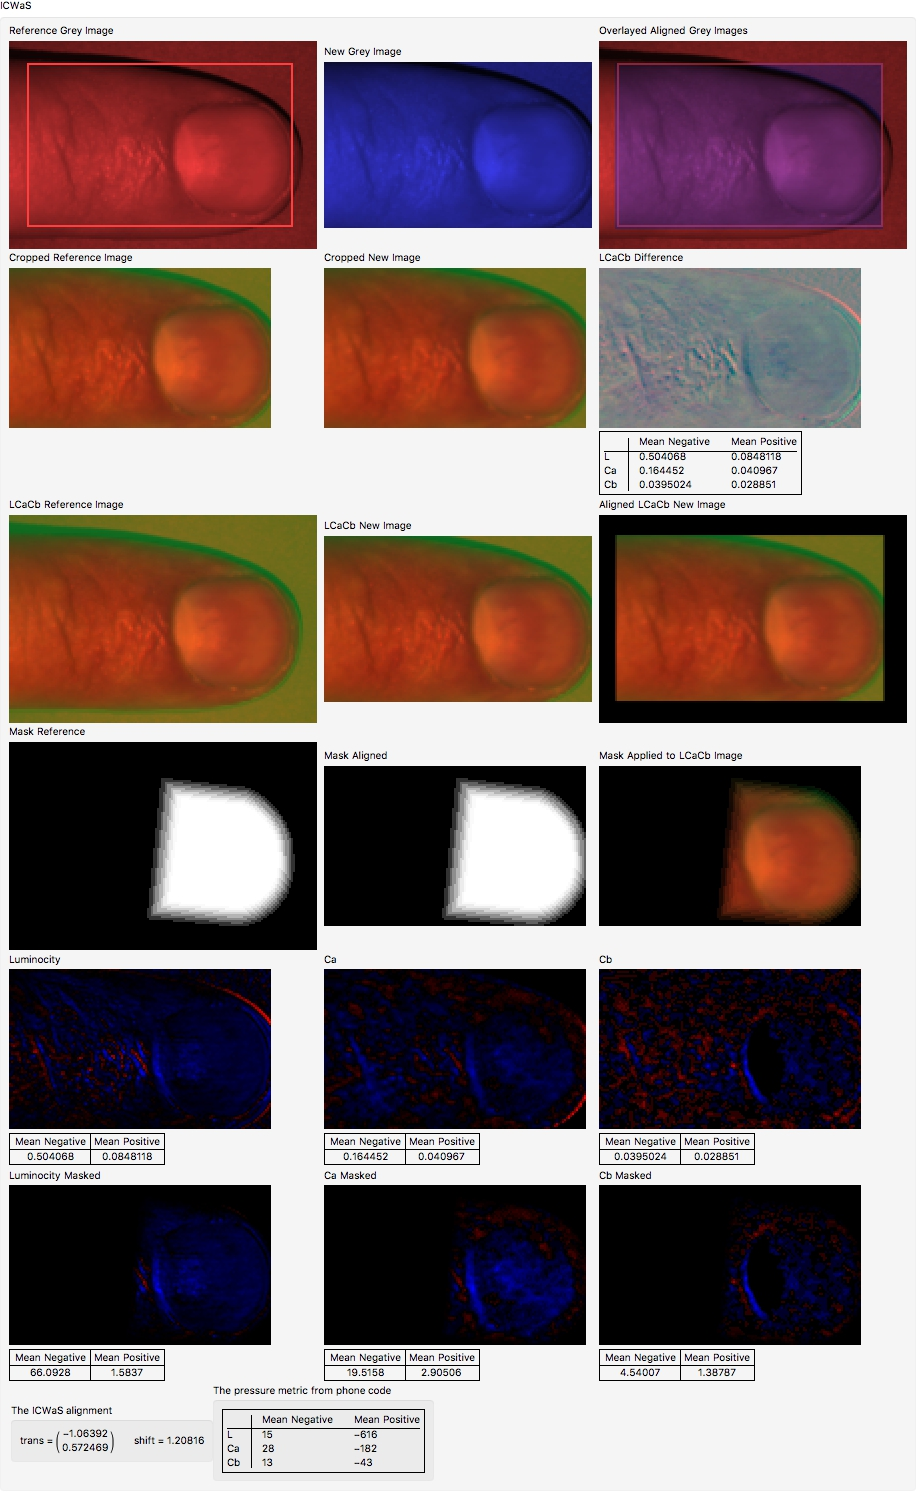
\includegraphics[width=0.95\textwidth]{Chapter4/Figs/ICWaS4.jpg}
%    \caption{ICWaS4}\label{fig:ICWaS4}
%\end{figure}


\section{The `Elliptical Fit' Method}\label{sec:EllipticalFitMethod}
Fitting an ellipse to a set of points is surprisingly difficult. The reason for this is outlined below.

To follow the standard linear algebra approach to least squares fitting, we need to decide upon a functional form for the fit, and thereby a basis set. For an ellipse, this basis set is $\chi= \left(x^2, x y, y^2, x, y, 1\right)$, which is a set of six free coefficients $ A^T=\left\{A_{\text{xx}},A_{\text{xy}},A_{\text{yy}},A_x,A_y,A_0\right\}$. However, to specify an ellipse, all that is needed is five numbers; the major and minor axes lengths $(a,b)$, the position $(x_0,y_0)$, and the orientation $\theta$. This is because the basis set includes lines, quadratics, parabolic and hyperbolic functions as well as elliptical functions as possible fits. An additional difficulty arises when we try to construct a cost function for an ellipse. Ideally, we wish to minimize the perpendicular distances of the points from the ellipse, but the calculation of the distance of a point from an ellipse is not straightforward, requiring the roots of a fourth degree polynomial to be found. Due to these complexities, several different methods have been proposed by different authors, but we will be focusing on two methods: The Approximate Mean Square (AMS)  proposed by (\cite{Taubin1991}), and the Direct least square (Direct) method by (\cite{Fitzgibbon1999}).


For the fingertip problem, there is also the added difficulty that the points are confined to one side of the ellipse so we have chosen methods which cope well with partially occluded ellipses. Both methods begin by forming the design matrix and then applying an additional constraint which restricts the fit to a family of curves. Both methods are formulated as generalized eigenvalue problems, avoiding the need for iterative methods.

The AMS method restricts the fit to parabolic, hyperbolic and elliptical curves by imposing the condition that $ A^T ( D_x^T D_x  +   D_y^T D_y) A = 1$ where the matrices $Dx$ and $Dy$ are the partial derivatives of the design matrix $D$ with respect to x and y. The matrices are formed row by row applying the following to each of the points in the set:
\begin{align*}
D(i,:)&=\left\{x_i^2, x_i y_i, y_i^2, x_i, y_i, 1\right\} &
D_x(i,:)&=\left\{2 x_i,y_i,0,1,0,0\right\} &
D_y(i,:)&=\left\{0,x_i,2 y_i,0,1,0\right\}
\end{align*}
The AMS method minimizes the cost function
\begin{equation*}
\epsilon ^2=\frac{ A^T D^T D A }{ A^T (D_x^T D_x +  D_y^T D_y) A^T }
\end{equation*}

The minimum cost is found by solving the generalized eigenvalue problem.

\begin{equation*}
 D^T D A = \lambda  \left( D_x^T D_x +  D_y^T D_y\right) A 
\end{equation*}

The Direct method confines the fit to ellipses by ensuring that $4 A_{xx} A_{yy}- A_{xy}^2 > 0$. The condition imposed is that $4 A_{xx} A_{yy}- A_{xy}^2=1$ which satisfies the inequality and as the coefficients can be arbitrarily scaled is not overly restrictive.

\begin{equation*}
\epsilon ^2= A^T D^T D A \quad \text{with} \quad A^T C A =1 \quad \text{and} \quad C=\left(\begin{matrix}
 0 & 0  & 2  & 0  & 0  &  0  \\ 
 0 & -1  & 0  & 0  & 0  &  0 \\ 
 2 & 0  & 0  & 0  & 0  &  0 \\ 
 0 & 0  & 0  & 0  & 0  &  0 \\ 
 0 & 0  & 0  & 0  & 0  &  0 \\ 
 0 & 0  & 0  & 0  & 0  &  0 
\end{matrix} \right)
\end{equation*}

The minimum cost is found by solving the generalized eigenvalue problem.

\begin{equation*}
 D^T D A = \lambda  \left( C\right) A 
\end{equation*}

The system produces only one positive eigenvalue $ \lambda$ which is chosen as the solution with its eigenvector $\mathbf{u}$. These are used to find the coefficients

\begin{figure}[p]
\centering
\subfloat[Comparison of the AMS and Direct ellipse fit methods for a complete ellipse][AMS and Direct methods both perform well with a set of points evenly distributed arround the ellipse. ]{
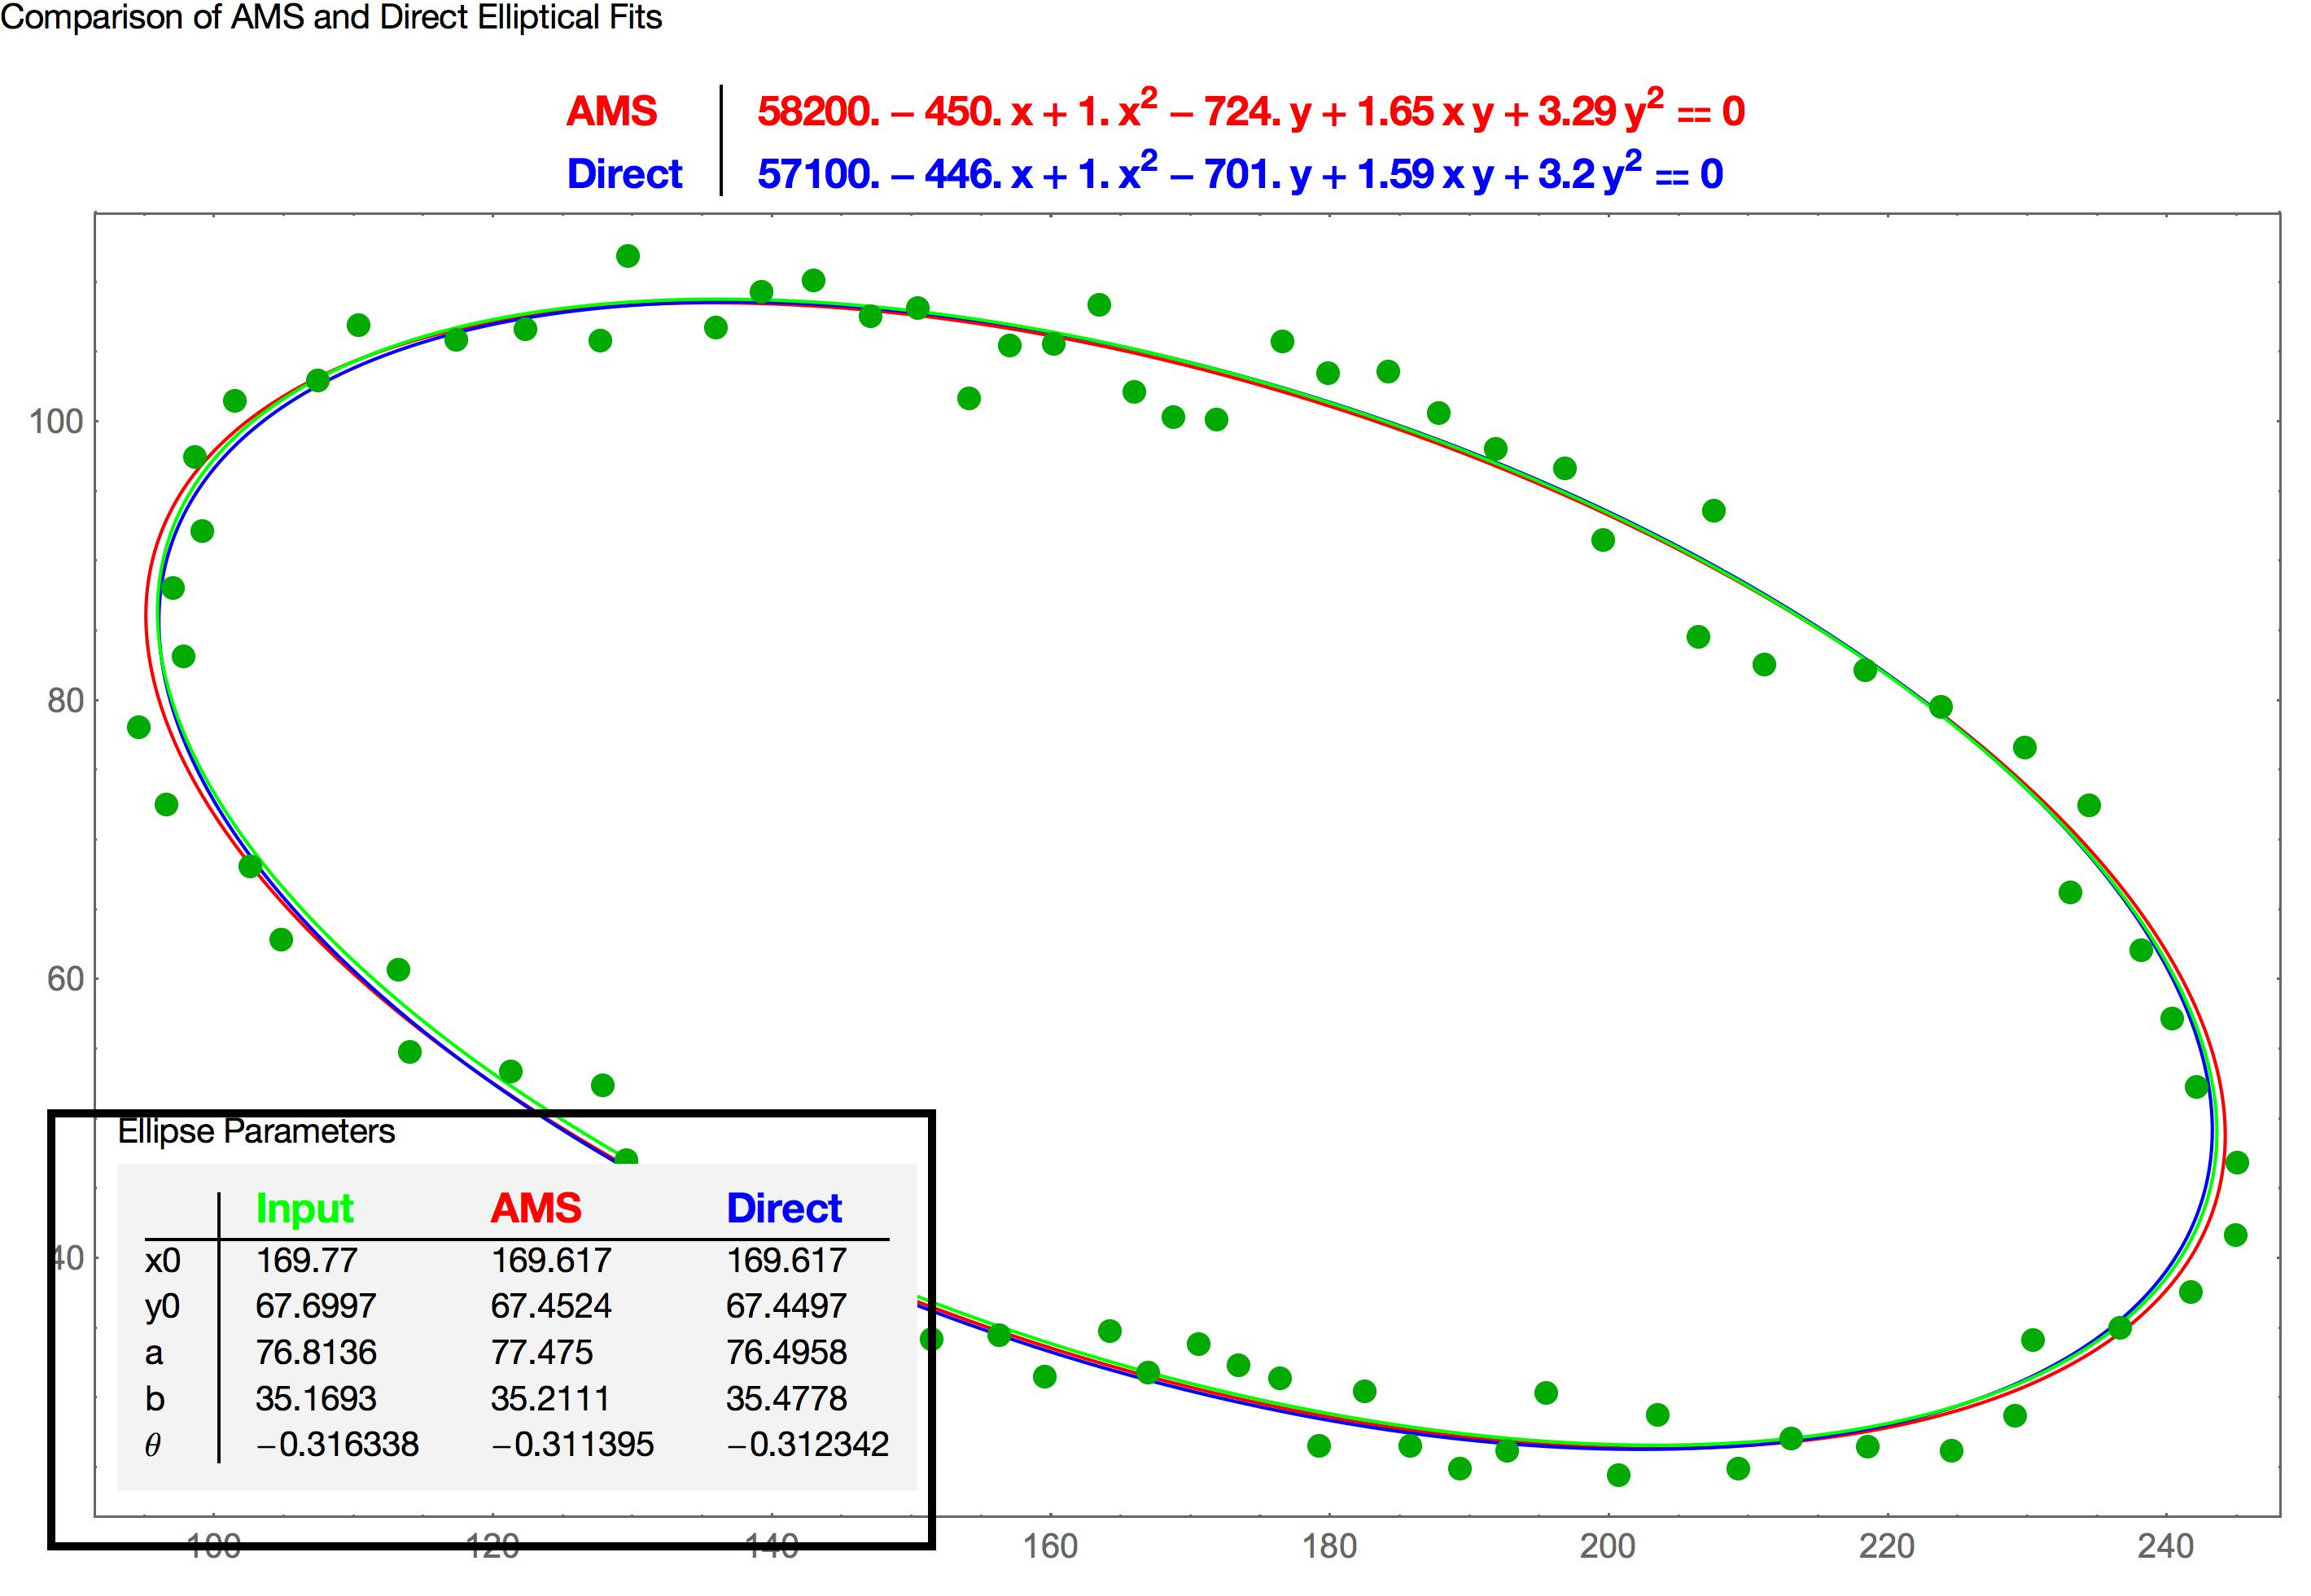
\includegraphics[width=0.98\textwidth]{Chapter4/Figs/EllipticalFitTestFull.jpg}
\label{fig:EllipseFitTestFull}}
\qquad
\subfloat[The AMS method sometimes produces a hyperbolic fit.][The AMS method sometimes produces a hyperbolic fit whilst the direct method always produces an ellipse]{
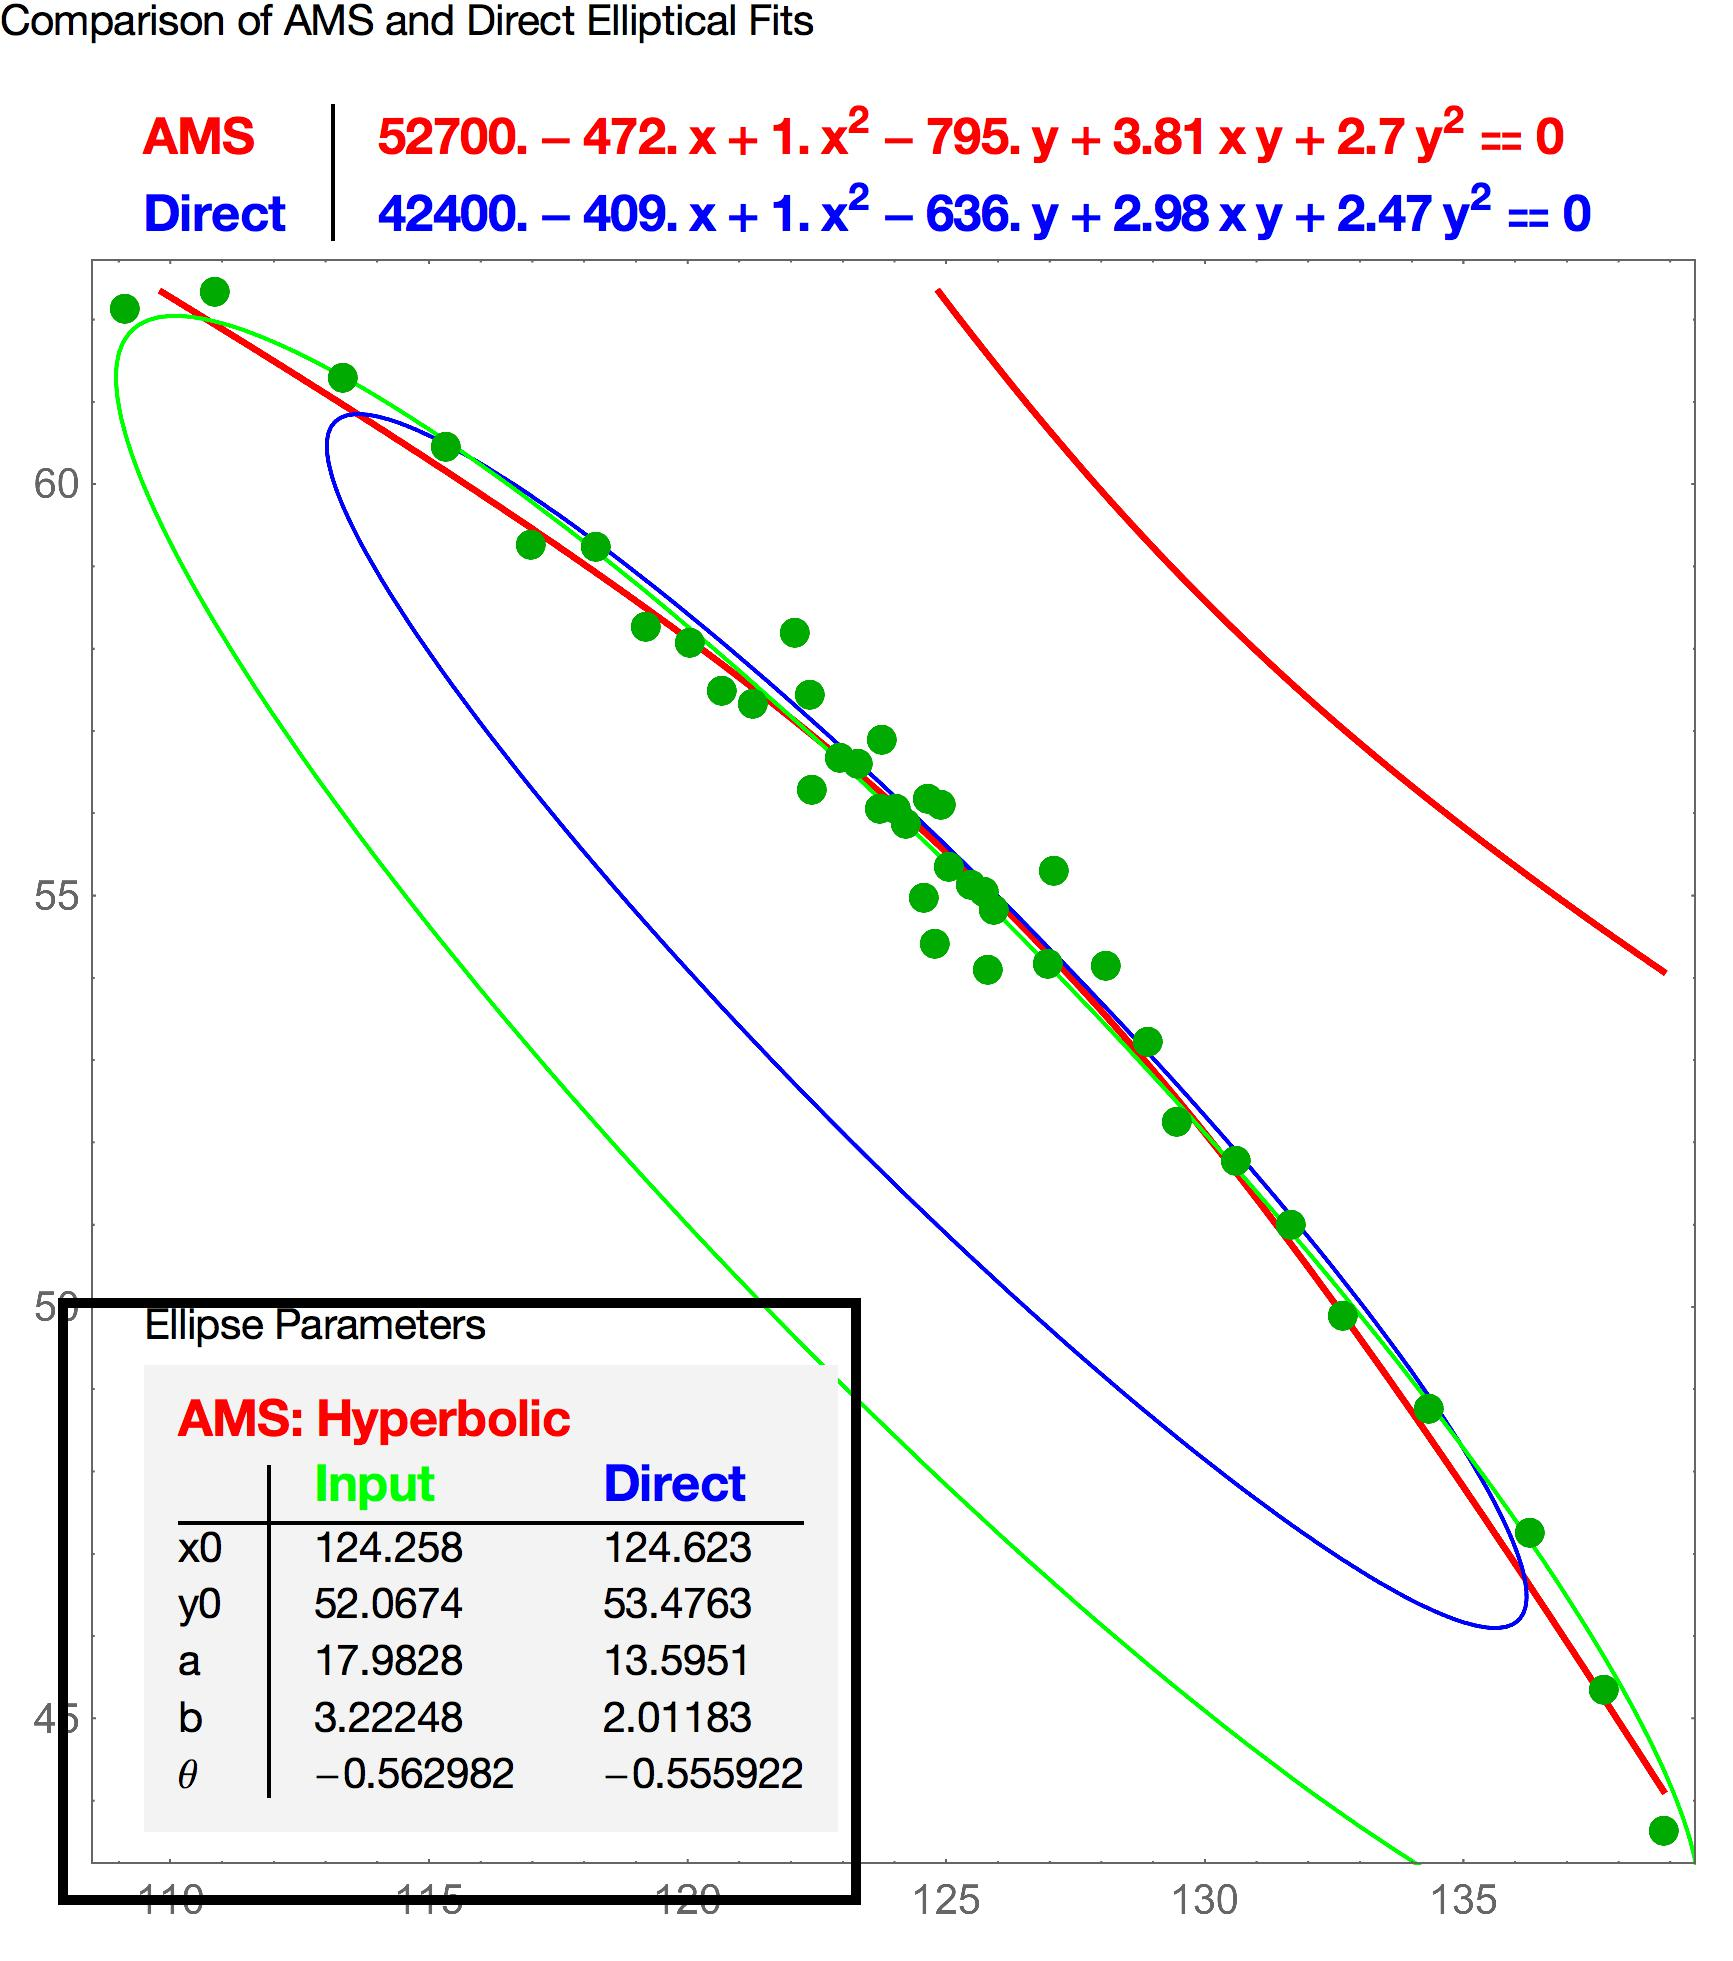
\includegraphics[width=0.47\textwidth]{Chapter4/Figs/EllipticalFitTest_Hyperbolic.jpg}
\label{fig:EllipseFitTestHalfHyperbolic}}
\quad
\subfloat[Comparison of the AMS and Direct ellipse fit methods for a half ellipse.][The AMS method better fits the extreme edge points in the data set resulting in the AMS method producing larger ellipses than the Direct method. The true ellipse is most often between the  two.]{
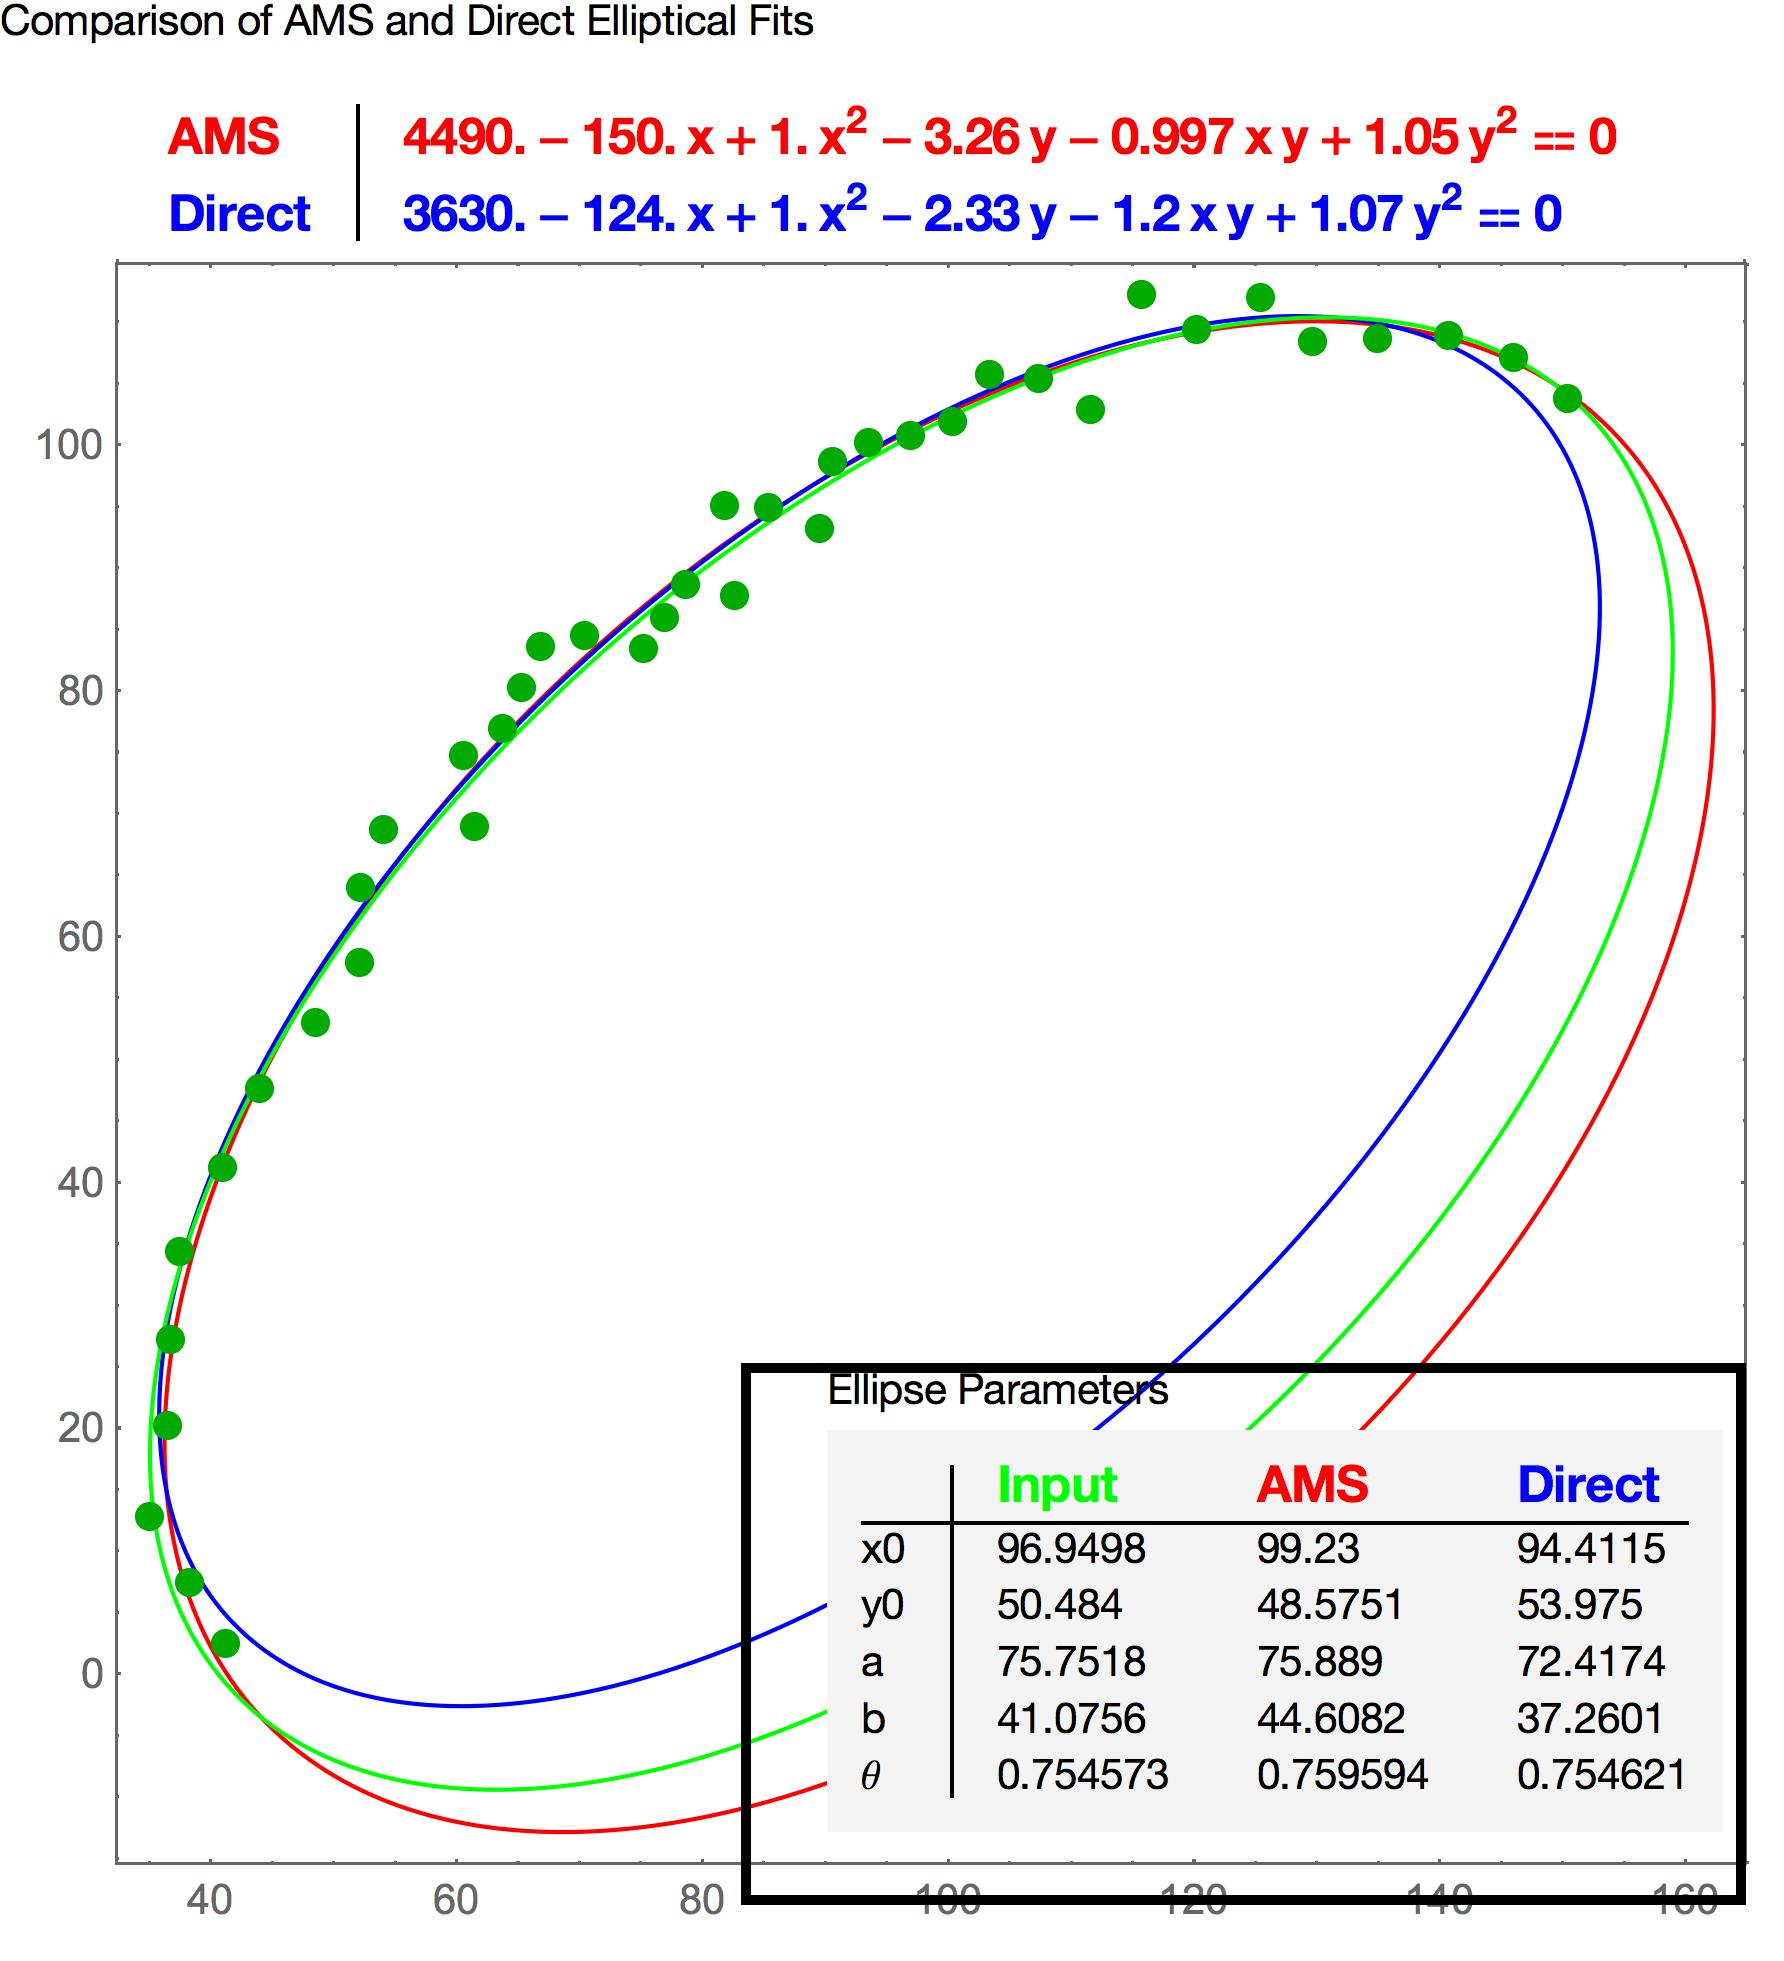
\includegraphics[width=0.47\textwidth]{Chapter4/Figs/EllipticalFitTest_DTA.jpg}
\label{fig:EllipseFitTestHalf}}
\caption{Comparison of the AMS and Direct ellipse fit methods.}
\label{fig:EllipseFitTest}
\end{figure}

\begin{equation*}
 A = \sqrt{\frac{1}{\mathbf{u}^T C \mathbf{u}}}  \mathbf{u}
\end{equation*}
The scaling factor guarantees that  $A^T C A =1$.

These methods were implemented in Mathematica for evaluation and in the OpenCV C++ code. Testing routines generated sample data with variable ellipse occlusion and noise around a randomly generated ellipse . The methods both produced good fits to complete ellipses Fig.\ref{fig:EllipseFitTestFull} and incomplete ellipses Fig.\ref{fig:EllipseFitTestHalf}. The AMS method was slightly better at fitting the extreme ends of the ellipse, generally producing a larger ellipse than the Direct method. Both methods accurately obtained the position and orientation. The AMS method occasionally produced a hyperbolic fit for very flat ellipses Fig \ref{fig:EllipseFitTestHalfHyperbolic}.


The largest computational effort in both methods is the determination of the $D^T D$ matrix. Once found, however, both methods can be used at relatively little extra computational cost. All Ellipses between the two can be considered as valid fits also. This suggests a method which allows for extra information to be used to refine the fit. In the case of the finger model this is the orientation, distal width and position from the parallel line fit. The ellipse between the two fits which most closely matches the extra information is chosen as the best fit.
\clearpage

\section{The `Isoscelian Trapezian' Fit}\label{sec:TrapezianFit}

Given three sets of points corresponding to the top, middle and bottom of an isosceles trapezium which is oriented so that the parallel sides are on the left and right, a fit can be found as follows:

\begin{enumerate}
\item A straight line fit to the midpoints is found giving start and end points along with an orientation.
\item The points are translated and rotated so that the first middle point is at the origin and the last middle point is on the x axis.
\item The bottom points are reflected about the x axis.
\item A single straight line is fitted to the top and reflected bottom points together.
\item Four points describing the trapezium are found and returned along with the orientation and position in the original coordinates.
\end{enumerate}

\section{The `Force Analogue Shape Detection' Method (FASDM)}\label{sec:ForceAnalogue}
\newcommand{\pos}{\mathbf{P}}
\newcommand{\F}{\mathbf{F}_i}
\newcommand{\Ft}{\mathbf{F}^\tau_i}
\newcommand{\dm}{\mathbf{d}^{m{\scriptscriptstyle dl} }_i}
\newcommand{\di}{\mathbf{d}^{i{\scriptscriptstyle mg} }_i}
\newcommand{\Mt}{\mathbf{\tau}_i}
The FASDM is one of the most straightforward --- if not the most straightforward --- shape alignment algorithms. Given a set of points, if we know a corresponding set of points on the the target shape model, we can find translation vectors between the points on the model $\dm$ and the points  on the image $\di$; the FASDM makes the analogue between these vectors and a force acting on that point on the model $\F=\di-\dm$. The position and orientation of the shape is then found by translating and rotating the model such that the 'force' acting upon it sums to zero. To facilitate the calculation the model is expressed in coordinates where the origin corresponds to the center of mass for the model.

It should be noted that other transformations can easily be included, however for the current purposes, rotation and translation are all that is required.
The translation vector $\F$ is found by taking the average of the force acting on the center of mass $\pos= \frac{1} {n} \sum_{i=1}^n \F$. 
Translating the model to this position allows the residual turning forces to be found $\Ft = \F - \pos$. 
The moment about the center of mass $\Mt$ is found simply by finding the magnitude of the outer product of the residual turning force $\Ft$ with the the point on the model $\dm$ thus $\Mt = \lVert \Ft \wedge \dm \rVert$. 
The rotation which would reduce the moment to zero is found by taking the angle between $\dm$ and $\dm+\Ft$.
The moment weighted average of these is the angle $\theta$ which will most reduce the total rotational moment $\mathbf{\tau} $. 

\begin{align*}
\theta &= \frac{1} {\mathbf{\tau}} \sum_{i=1}^{n} \Mt \theta_i &
\theta_i &=  \arccos \left(\frac{\dm \cdot (\dm+\Ft)}{\lVert \dm \rVert \lVert \dm+\Ft \rVert}\right)  &
\mathbf{\tau} &= \sum_{i=1}^{n} \Mt \\
\pos &= \frac{1} {n} \sum_{i=1}^n \F &
  &=  \arccos \left(\frac{\dm \cdot (\di - \pos)}{\lVert \dm \rVert \lVert \di - \pos \rVert}\right)  &
\Mt &= \lVert (\di - \pos) \wedge \dm \rVert
\end{align*}

\begin{figure}[h!]
  \centering
    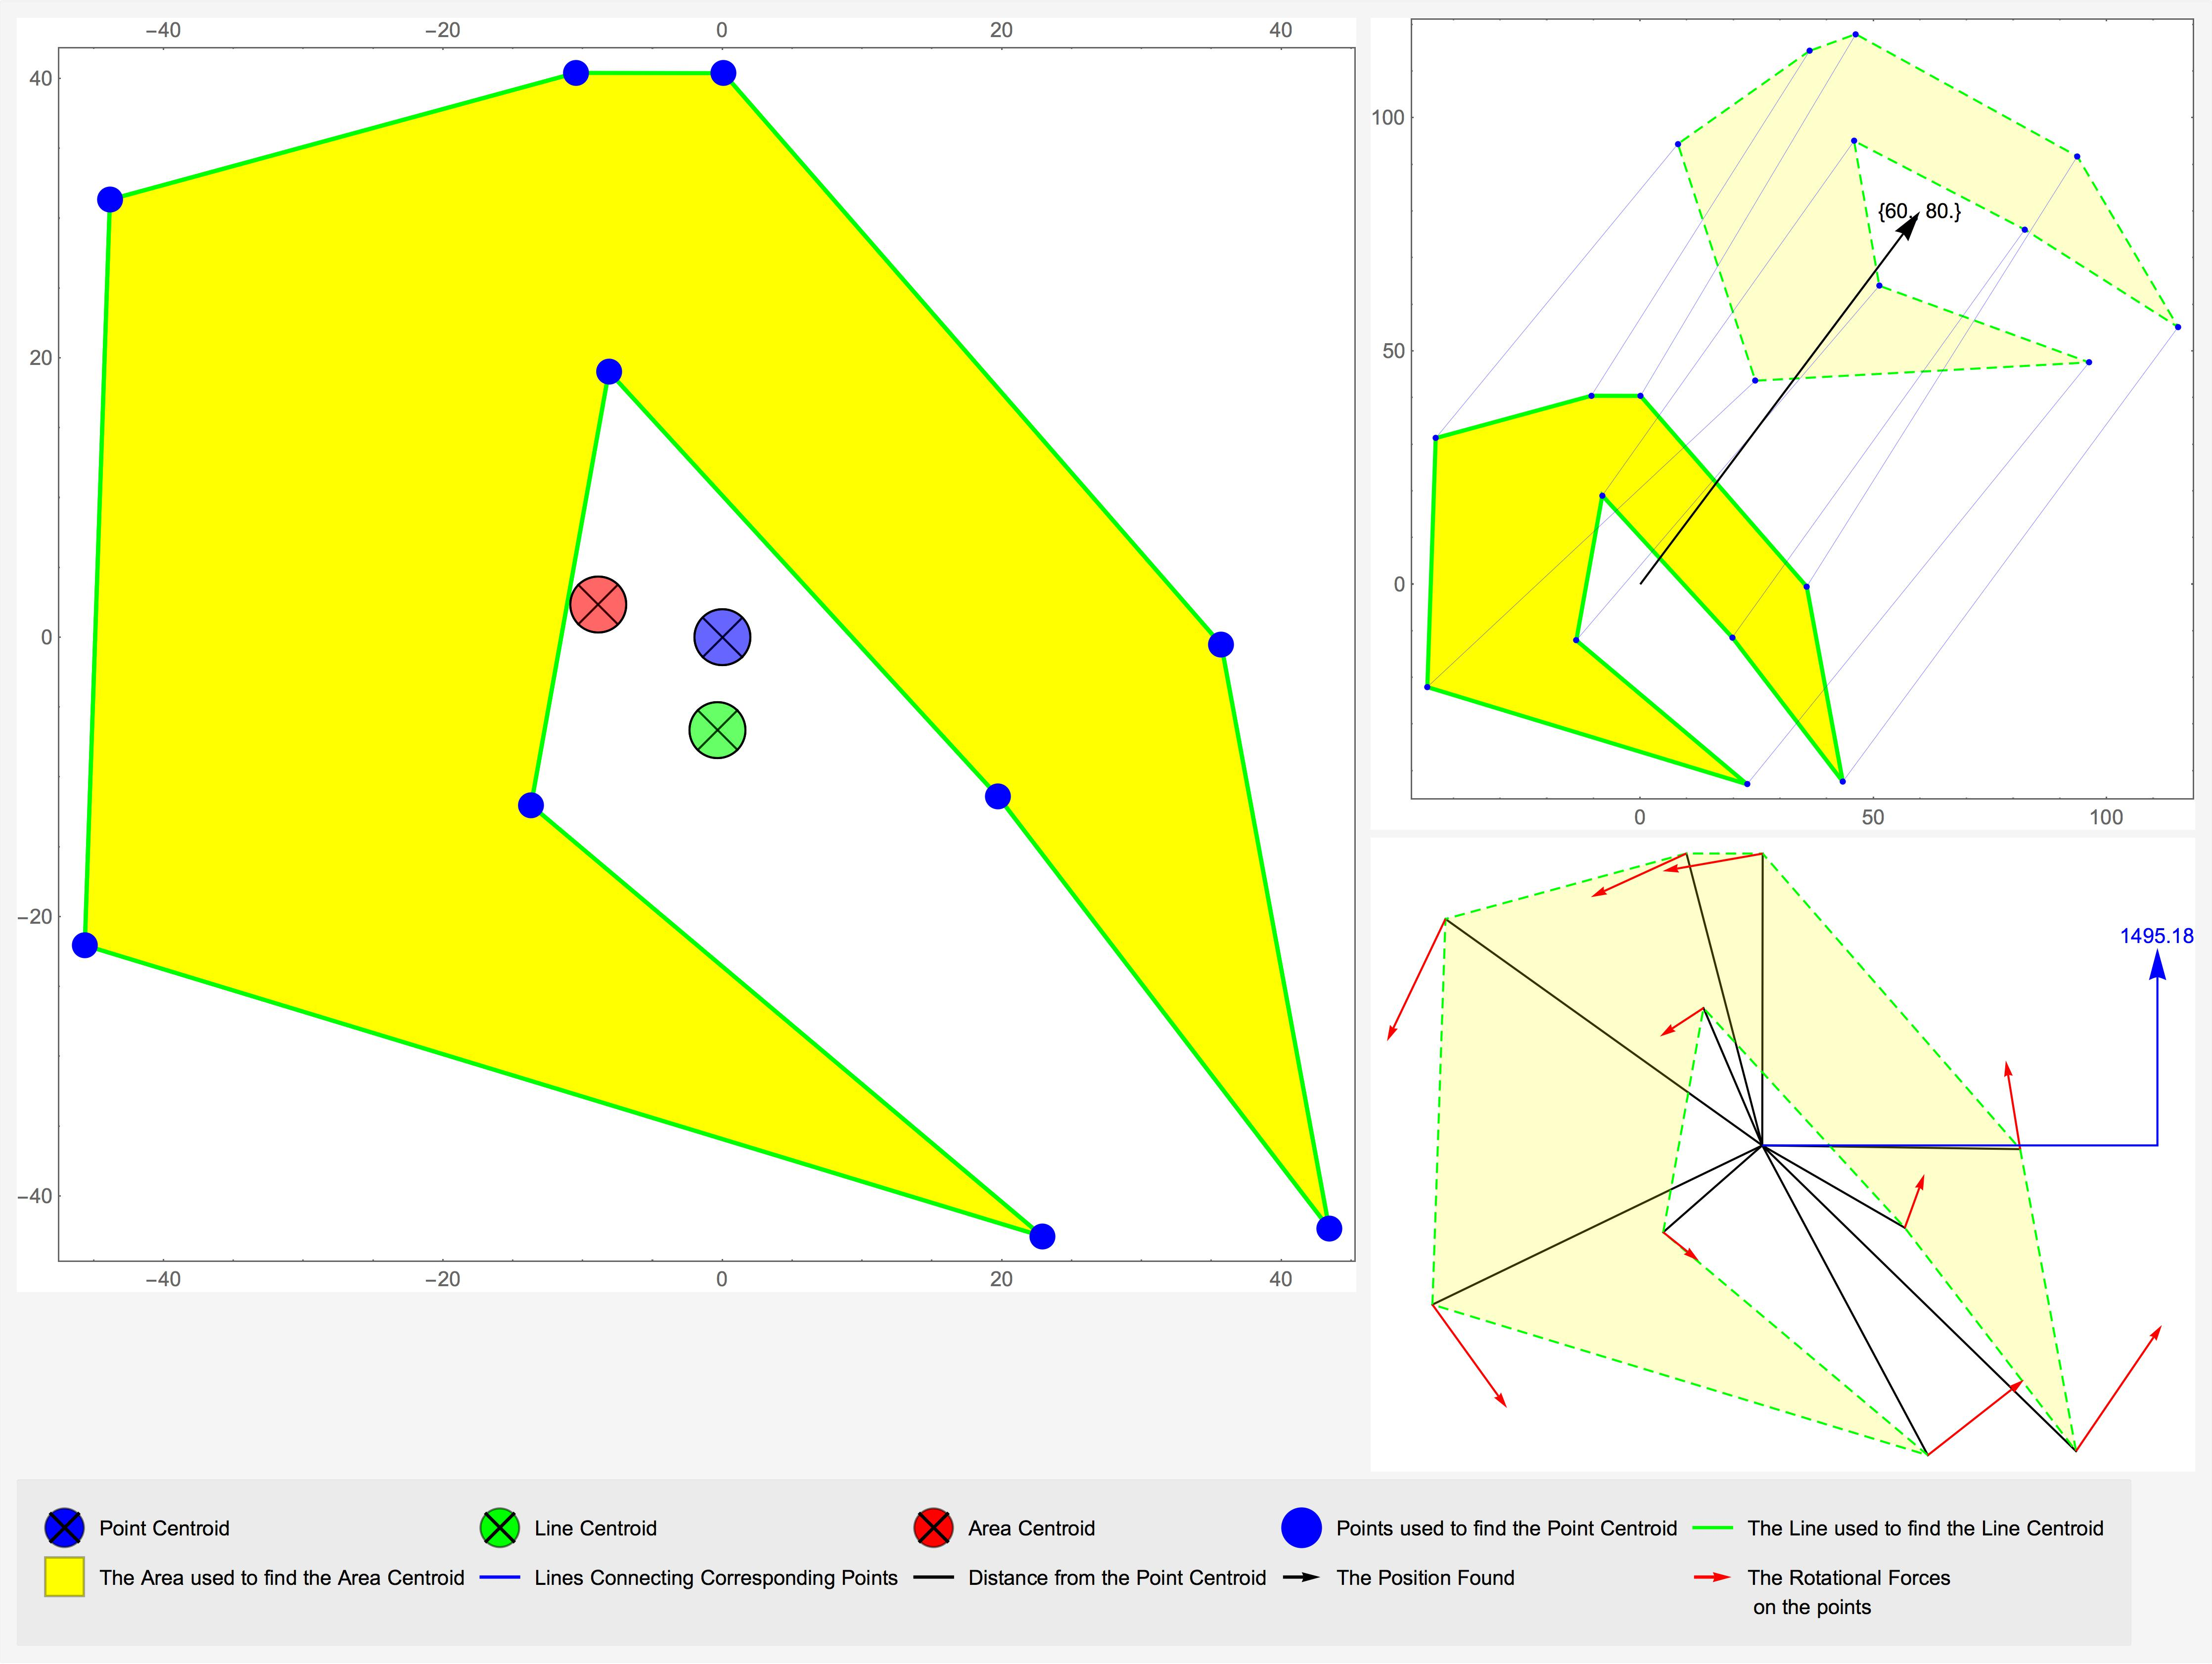
\includegraphics[width=0.95\textwidth]{Chapter4/Figs/Random_Polygon_Centroids.jpg}
    \caption{Random Polygon Centroids.}\label{fig:RandomPolygonCentroids}
\end{figure}

\begin{figure}[h!]
  \centering
    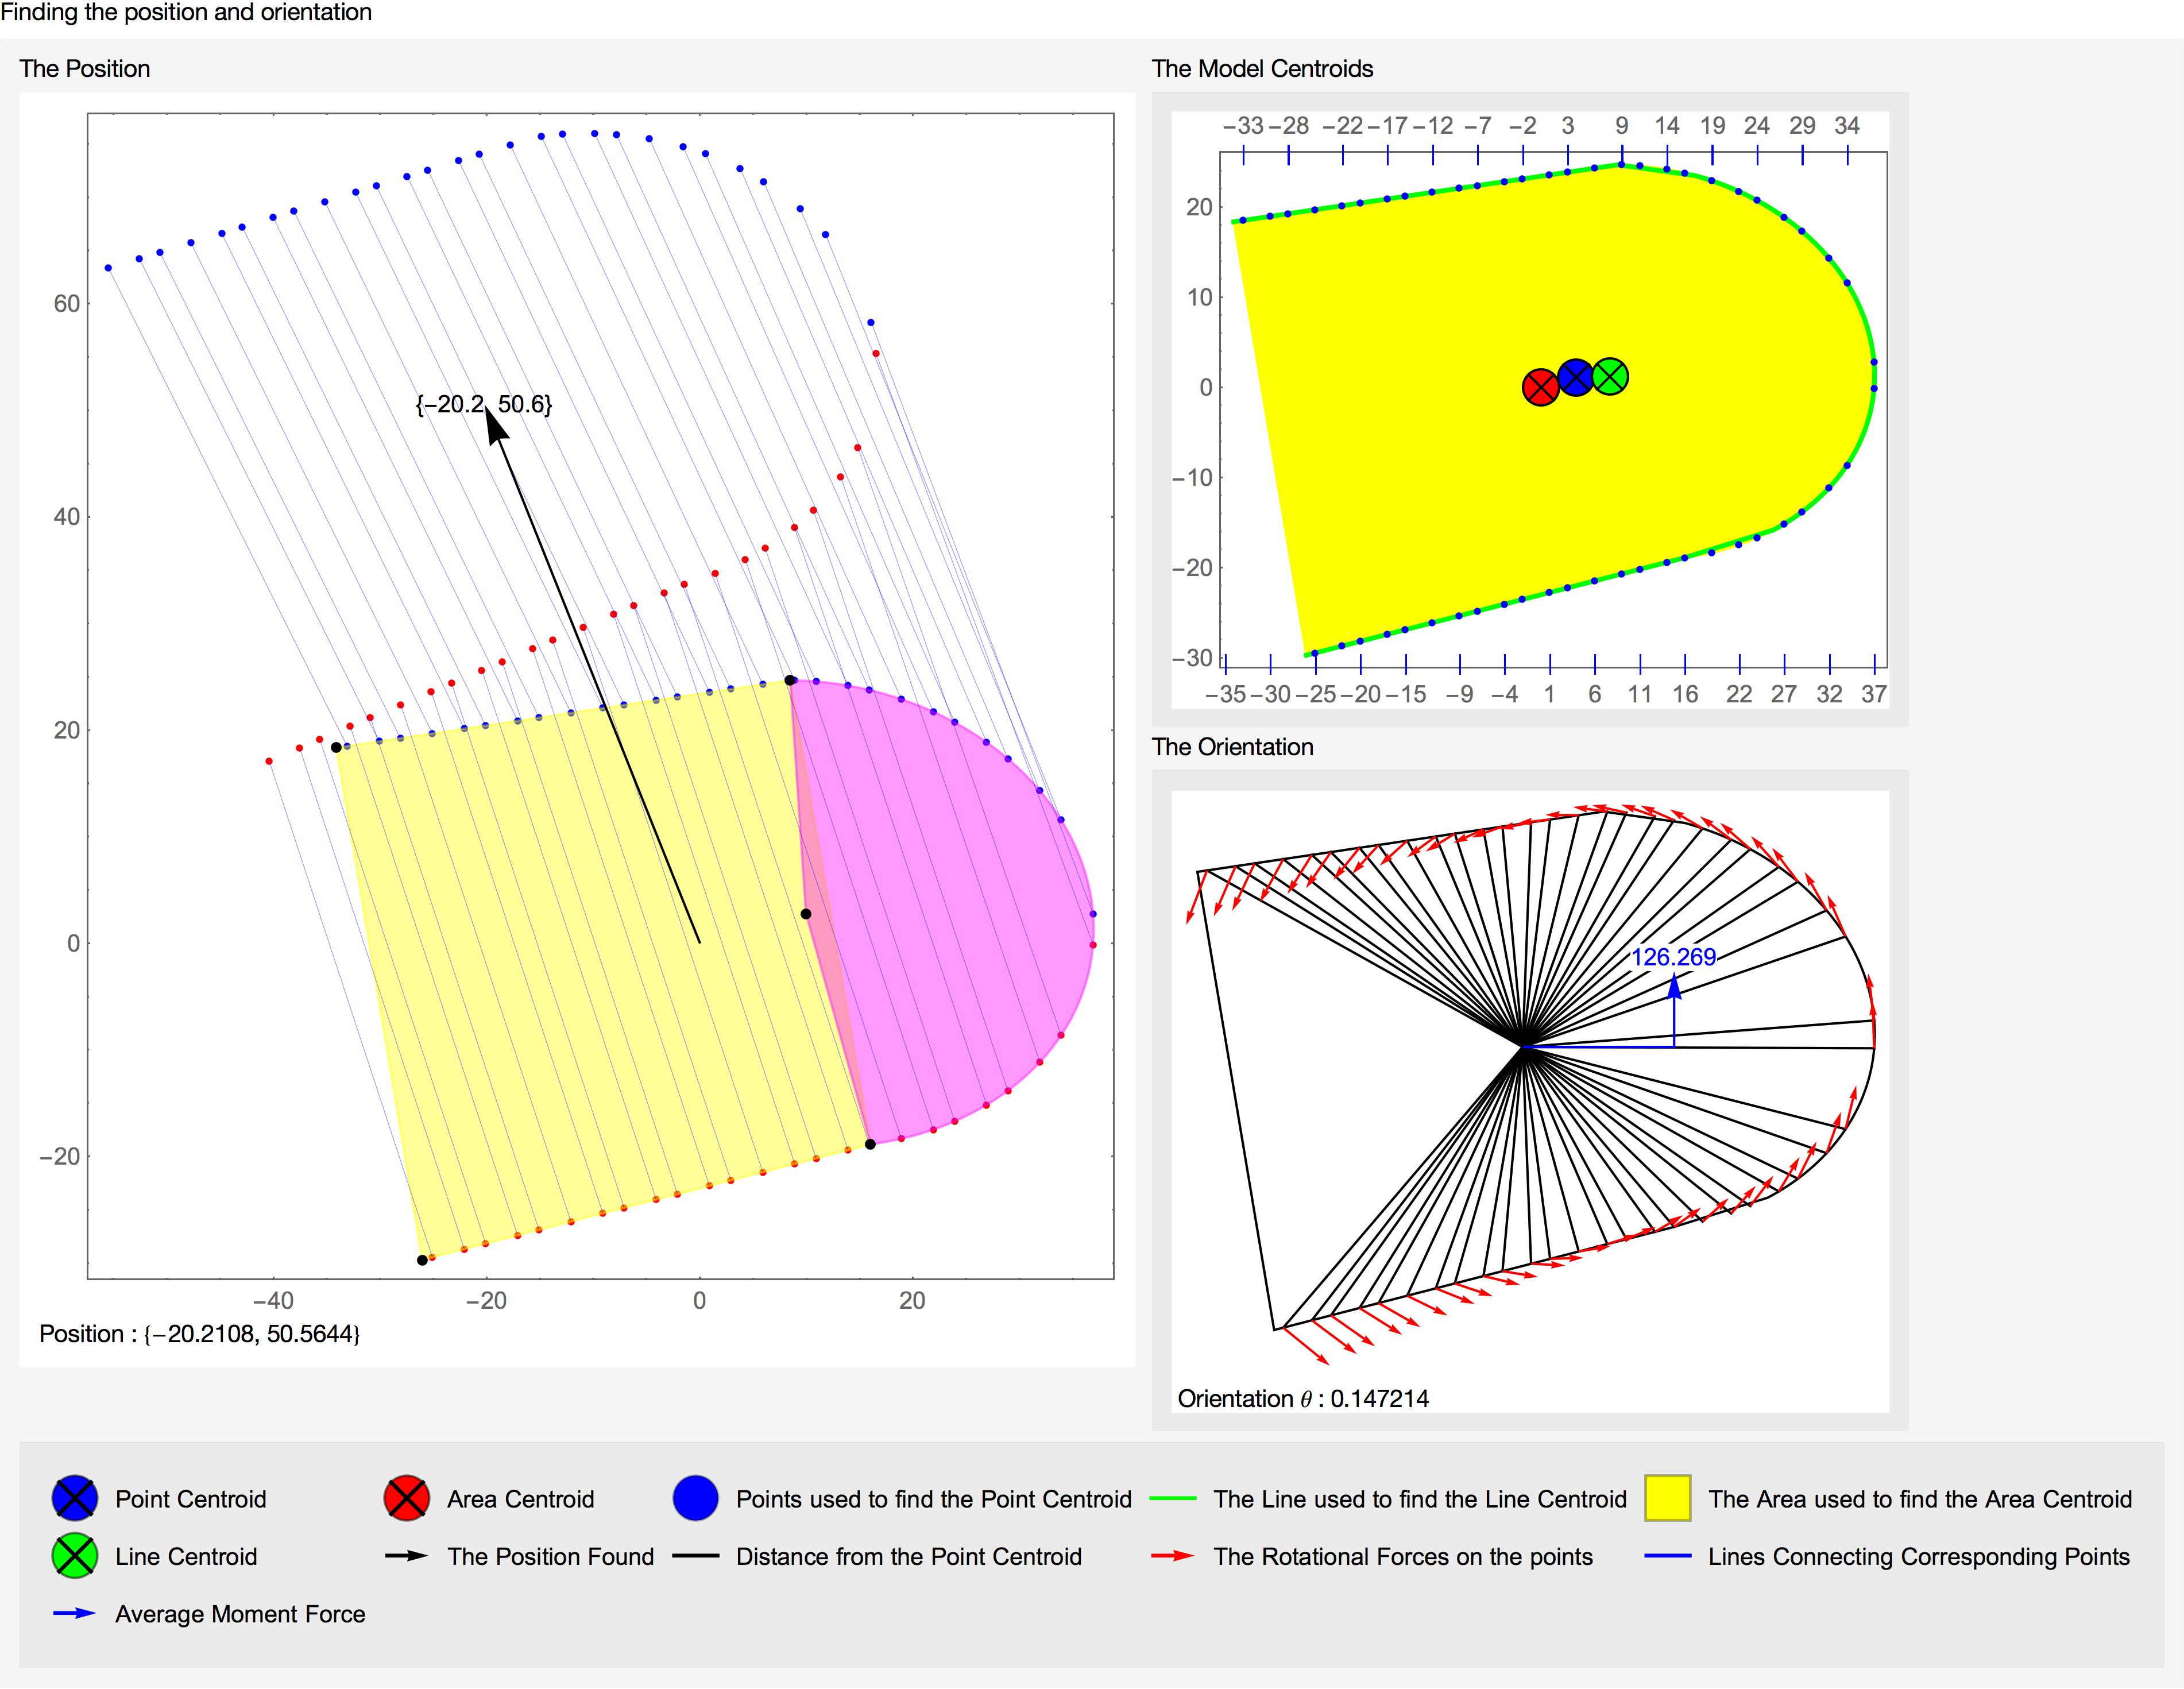
\includegraphics[width=0.95\textwidth]{Chapter4/Figs/Exagerated_Model_Centroids_With_Pos_Orientation.jpg}
    \caption{Position and Orientation.}\label{fig:ExaggeratedPositionAndOrientation}
\end{figure}

 Mathematically and algorithmically, there are three points which may be considered the center of mass: the centroid of the area of the model, which is where the center of mass would be if the model were a a flat, uniform sheet; the centroid of the perimeter of the model, which is the center of mass would be if the model were constructed using wire along the perimeter; and the arithmetic average of the points of interest defined on the perimeter of the model. (See Figure \ref{fig:RandomPolygonCentroids}.) The choice for the analogue of the center of mass depends upon the algorithm used. For a method which returns points radially distributed about a point in the model would favor the area centroid; a method which returned points relatively evenly distributed along the perimeter would naturally favor the perimeter centroid method; and a method which returned points of interest would favor the point centroid method. (There's no guarantee the points of interest would be distributed in any relation to the shape-based centroids.) An example fingertip model centroid and FASDM method can be seen in Figure \ref{fig:ExaggeratedPositionAndOrientation}.
 
 The Filament Fill algorithm returns a set of points distributed linearly around the perimeter. The appropriate FASDM method is therefore a point-based centroid found by generating points along the shape perimeter which are equally-spaced perpendicular projections from the shape axis.

\chapter{iPhone Camera Setup}\label{sec:iPhoneCameraSetup}
Quite later on in development, an iOS update was released which allows in-code control of camera properties, such as focus, exposure and white point color balance. Because the code does per-pixel comparisons and assumes that the color values remain constant, the first thing this allows us to do is fix the exposure, the white point and the focus such that, as the code is tracking the digit and tracking the blood flow, the algorithm isn't thrown off by the phone deciding to suddenly changing the camera properties. 

Initially, a simple routine was added which simply fixed these camera properties before starting the tracking. However, it was apparent that we could take advantage of the camera control features to produce a better result. First, we needed to be able to perform a metric for how good the camera settings are for tracking. Initially, this metric was taken using the whole image. Taking the classified image, the metric was formed by taking a weighted sum of the classified image pixel values; the metric scored values of 0 and 3 positively and values of 1 and 2 negatively, the idea being to promote camera settings which result in a classified image which rewards certainty.

However, the problem with this approach is that if the camera properties are set with, say, a very low exposure, the image is almost entirely black and the classified image is certain that there isn't a finger in the picture, regardless of the reality, so this metric is scored highly. To combat this, the app allows two regions to be selected in the frame, one which definitely contains skin, and one which definitely does not. We then have two separate metrics for the skin region; values of 2 and 3 are scored highly, while values of 0 and 1 are scored negatively, and conversely for the skinless region.

After all this work, we have three metrics: one which rewards correctly identifying skin, one which rewards correctly identifying background, and one which rewards overall certainty. The final metric which was returned in the camera calibration is the weighted sum of these three metrics; the skin and the background identification metrics given a slightly higher weighting than the overall certainty.

\clearpage

\section{Setting the Exposure}\label{sec:SettingTheExposure}
\begin{figure}[h!]
  \centering
    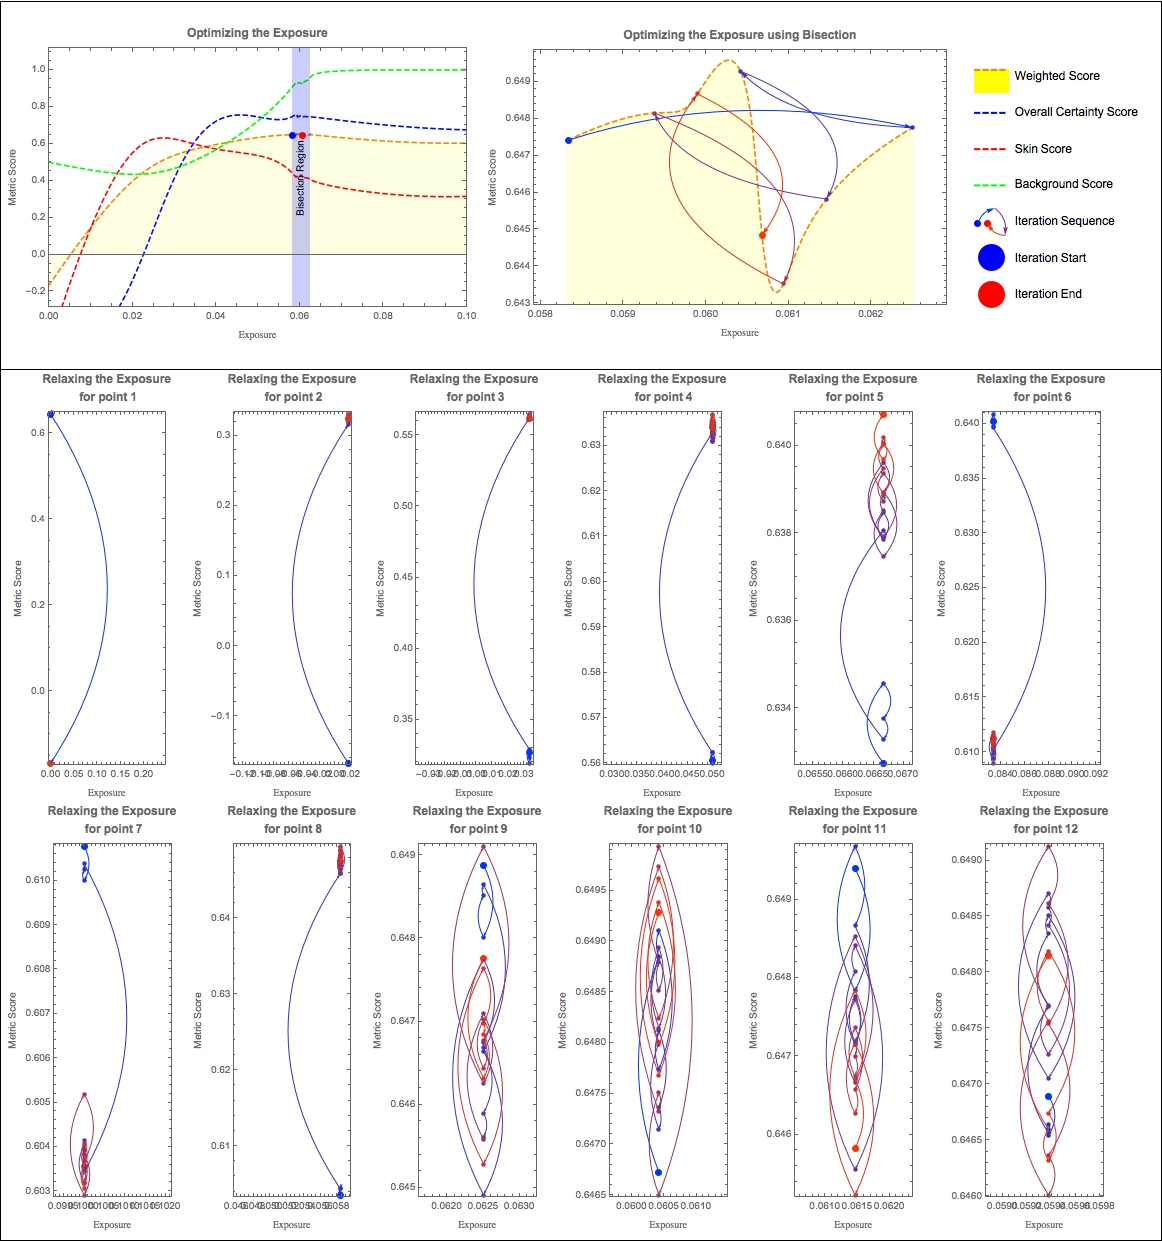
\includegraphics[width=0.95\textwidth]{Chapter4/Figs/exposureGraphic1.jpg}
    \caption{Optimization of the exposure for the iPhone camera.}\label{fig:ExposureGraphic1}
\end{figure}
To find the optimal exposure, the code first picks a handful of values between a minimum and maximum exposure and evaluates the metric at these values. This is done by setting the exposure waiting in-code for a few microseconds for the camera to finish adjusting and then evaluating the metric. This is necessary because the camera properties are set in a different thread to the tracking algorithm's thread. A bisection algorithm is then used to refine the optimal exposure (Figure  \ref{fig:ExposureGraphic1}).


